\documentclass[10pt]{article}
\pdfoutput=1 

\addtolength{\oddsidemargin}{-.875in}
\addtolength{\evensidemargin}{-.875in}
\addtolength{\textwidth}{1.75in}

\addtolength{\topmargin}{-.875in}
\addtolength{\textheight}{1.75in}

\openup 1em

%macro for commenting
\usepackage{color}
\newcommand{\leo}[1]{{\color{blue}{\it leo: #1}}}

\newcommand{\Xbeta}{ X_i \theta}
\newcommand{\xbeta}{ x_i \theta}
\newcommand{\xbetaij}{ x_{ij}^T \theta}
\newcommand{\sgamma}{s_{ij}^T\gamma_i}

\usepackage[round]{natbib}

\usepackage{rotating}
\usepackage{graphicx}
\usepackage{subcaption}

\usepackage{float}


\usepackage{amsthm,amsmath} 
\usepackage{amssymb}
\usepackage{subcaption}

\newtheorem{theorem}{Theorem}
\newtheorem{lemma}{Lemma}
\newtheorem{corollary}{Corollary}
\newtheorem{remark}{Remark}


\usepackage{algorithm}
\usepackage{algpseudocode}

\usepackage{mhequ}
\newcommand{\be}{\begin{equs}}
\newcommand{\ee}{\end{equs}}
\newcommand{\bb}[1]{\mathbb{#1}}
\newcommand{\mc}[1]{\mathcal{#1}}
\DeclareMathOperator{\Binom}{Binomial}
\DeclareMathOperator{\No}{No}
\DeclareMathOperator{\PG}{PG}
\DeclareMathOperator{\IG}{Inverse-Gamma}
\DeclareMathOperator{\Ga}{Gamma}
\DeclareMathOperator{\Bern}{Bernoulli}
\DeclareMathOperator{\U}{Uniform}
\DeclareMathOperator{\Poi}{Poisson}
\DeclareMathOperator{\NB}{NB}
\DeclareMathOperator{\cov}{cov}
\DeclareMathOperator{\var}{var}
\DeclareMathOperator{\diag}{diag}
\DeclareMathOperator{\Diag}{Diag}
\DeclareMathOperator{\bigO}{\mc O}
\newcommand{\James}[1]{\textcolor{blue}{#1}}


\thispagestyle{empty}
\baselineskip=28pt

\title
{{Calibrated Data Augmentation for Scalable \\ Markov Chain Monte Carlo}}


\author{
     Leo L. Duan,
     James E. Johndrow,
     David B. Dunson
    % \textsuperscript{*}\footnotemark[2]\and
}

 
\begin{document}
    
\maketitle

{\bf Abstract:} Data augmentation is a common technique for building tuning-free Markov chain Monte Carlo algorithms. Although these algorithms are very popular, 
autocorrelations are often high in large samples, leading to poor computational efficiency.  This phenomenon has been attributed to a discrepancy between Gibbs step sizes and the rate of posterior concentration.  In this article, we propose a family of calibrated data augmentation algorithms, which adjust for this discrepancy by inflating Gibbs step sizes  while adjusting for bias.  A Metropolis-Hastings step is included to account for the slight discrepancy between the stationary distribution of the resulting sampler and the exact posterior distribution.  The approach is applicable to a broad variety of existing data augmentation algorithms, and we focus on three popular models: probit, logistic and Poisson log-linear.  Theoretical support is provided and dramatic gains are shown in applications.
\vskip 12pt

%\baselineskip=12pt
%\par\vfill\noindent
{\noindent  KEY WORDS:  Bayesian probit; Bayesian logit; Big $n$; Data Augmentation; Maximal Correlation; Polya-Gamma.}
%\par\medskip\noindent
%\clearpage\pagebreak\newpage
\pagenumbering{arabic}

\section{Introduction}

With the deluge of data in many modern application areas, there is pressing need for scalable computational algorithms for inference from such data, including uncertainty quantification (UQ).  Somewhat surprisingly, even as the volume of data increases, uncertainty often remains sizable.  Examples in which this phenomenon occurs include financial fraud detection \citep{ngai2011application}, disease mapping \citep{wakefield2007disease} and online click-through tracking \citep{wang2010click}.  Bayesian approaches provide a useful paradigm for quantifying uncertainty in inferences and predictions in these and other settings.

The standard approach to Bayesian posterior computation is Markov chain Monte Carlo (MCMC) and related sampling algorithms. Non-sampling alternatives, such as variational Bayes, tend lack general accuracy guarantees. However, it is well known that conventional MCMC algorithms often scale poorly in problem size and complexity. Due to its sequential nature, the computational cost of MCMC is the product of two factors: the evaluation cost at each sampling iteration and the total number of iterations needed to obtain an acceptably low Monte Carlo error. The latter is related to the properties of the Markov transition kernel; we will refer to this informally as the \emph{mixing properties} of the Markov chain. 

In recent years, a substantial literature has developed focusing on decreasing computational cost per iteration (\cite{minsker2014robust,srivastava2015wasp,conrad2015accelerating} among others), mainly through accelerating or parallelizing the sampling procedures at each iteration. Moreover, myriad strategies for improving mixing have been described in the literature. For Metropolis-Hastings (M-H) algorithms, improving mixing is usually a matter of contructing a better proposal distribution. An important difference between M-H and Gibbs is that one has direct control over step sizes in M-H through choice of the proposal, while Gibbs step sizes are generally not tunable; on the other hand, finding a good proposal for multi-dimensional parameters in M-H is significantly more challenging compared to Gibbs sampling. Thus, improving mixing for Gibbs has historically focused on decreasing autocorrelation by changing the update rule itself, for example by parameter expansion (PX), marginalization, or slice sampling.\footnote{Although strictly speaking, slice sampling is just an alternative approach to sampling from a full conditional distribution, in practice, it is often an alternative to data augmentation, so that using a slice sampling strategy results in the removal of a data augmentation step from an alternative Gibbs sampler.} 

The theory literature on behavior of MCMC for large $n$ and/or $p$ is arguably somewhat limited. Many authors have focused on studying mixing properties by showing 
an ergodicity condition, such as geometric ergodicity \citep{roberts2004general,meyn2012markov}. This generally yields bounds on the convergence rate and spectral gap of the Markov chain, but \cite{rajaratnam2015mcmc} observe that in many cases, these bounds converge to zero exponentially fast in $p$ or $n$, so that no meaningful guarantee of performance for large problem sizes is provided by most existing bounds. In the probability literature, a series of papers have developed an analogue of Harris' theorem and ergodic theory for infinite-dimensional state spaces \citep{hairer2011asymptotic}. Recent work verifies the existence of MCMC algorithms for computation in differential equation models with dimension-independent spectral gap \citep{hairer2014spectral}. In this example, the algorithm under consideration is an M-H algorithm, and it is clear that the proposal must be tuned very carefully to achieve dimension independence. Other work has studied the properties of the limiting differential equation that describes infinite-dimensional dynamics of MCMC.

A recent paper (\cite{johndrow2016inefficiency}) studies popular data augmentation algorithms for posterior computation in probit \citep{albert1993bayesian} and logistic  \citep{polson2013bayesian} models, showing that the algorithms fail to mix in large sample sizes when the data are imbalanced. An important insight is that the performance can be largely explained by a discrepancy between the rate at which Gibbs step sizes and the width of the high-probability region of the posterior converge to zero as the sample size increases. Thus, since Gibbs step sizes are generally not tunable, slow mixing is likely to occur as the sample size grows unless the order of the step size happens to match the order of the posterior width. This implies that if a way to directly control the step sizes of the Gibbs sampler could be devised, it would be possible to make the mixing properties of the sampler insensitive to sample size by scaling the step sizes appropriately. This is similar to the conclusion of \cite{hairer2014spectral}, except in this case, we have growing $n$ instead of growing $p$.

In this article, we propose a method for tuning Gibbs step sizes by introducing auxiliary parameters that change the variance of full conditional distributions for one or more parameters. Although we focus on data augmentation algorithms for logit, probit, and Poisson log-linear models, in principle the strategy can be applied more generally to align Gibbs step sizes with the size of the space being explored. As these ``calibrated'' data augmentation algorithms alter the invariant measure, one can use the Gibbs step as a highly efficient M-H proposal, thereby recovering the correct invariant, or view the resulting algorithm as a perturbation of the original Markov chain.  In this article, we focus on the former strategy, providing theoretical support and showing very substantial practical gains in computational efficiency attributed to our calibration approach.

\section{Calibrated Data Augmentation}

Data augmentation Gibbs samplers alternate between sampling  latent data $z$ from their conditional posterior distribution given model parameters $\theta$ and observed data $y$, and sampling parameters $\theta$ given $z$ and $y$; either of these steps can be further broken down into a series of full conditional sampling steps but we focus for simplicity on algorithms of the form: 
\be \label{eq:da}
z \mid \theta, y &\sim \pi(z;\theta,y) \\
\theta \mid z,y &\sim f(\mu(z),\Sigma(z)),
\ee
where $f$ belongs to a location-scale family, such as the Gaussian.  Popular data augmentation algorithms are designed so that both of these sampling steps can be conducted easily and efficiently; e.g., sampling the latent data for each subject independently and then drawing $\theta$ simultaneously (or at least in blocks) from a multivariate Gaussian or other standard distribution.  This effectively avoids the need for tuning, which is a major issue for Metropolis-Hastings algorithms, particularly when $\theta$ is high-dimensional.
Data augmentation algorithms are particularly common for generalized linear models (GLMs), with $\bb E(y_i \mid x_i, \theta) = g^{-1}(x_i \theta)$ and a conditionally Gaussian prior distribution chosen for $\theta$. We focus in particular on Poisson log-linear, binomial logistic, and binomial probit as motivating examples.

\subsection{Initial example: Probit with improper prior}
We introduce our calibration approach through a binomial probit model example: 
\be
y_i \sim \Bern(p_i), \quad p_i = \Phi(x_i \theta),
\ee
with improper prior $\pi(\theta) \propto 1$. The basic data augmentation algorithm \citep{tanner1987calculation,albert1993bayesian} has the update rule
\be
z_i \mid \theta, x_i, y_i &\sim \left\{ \begin{array}{cc} \No_{[0,\infty)}(x_i \theta,1) & \text{ if } y_i = 1 \\ \No_{(-\infty,0]}(x_i \theta,1) & \text{ if } y_i = 0 \end{array} \right. \\
\theta \mid z, x, y &\sim \No((X'X)^{-1} X'z, (X'X)^{-1}),
\ee
where $\No_{[a,b]}(\mu,\sigma^2)$ is the normal distribution with mean $\mu$ and variance $\sigma^2$ truncated to the interval $[a,b]$.  %\cite{johndrow2016inefficiency} found that this algorithm has very poor mixing in imbalanced large data settings.  To solve this problem, 
We propose to make the Gibbs step sizes tunable by introducing an auxiliary parameter $r_i$ multiplying the variance of $z_i$, while also reducing the bias caused by $r_i$ through adjusting the mean by another auxiliary parameter $b_i$.  These adjustments yield 
\be
\mbox{pr}(y_i = 1 | \theta, x_i, r_i, b_i) = \int_{0}^{\infty} \frac{1}{\sqrt{2 \pi r_i} } \exp\left(-\frac{(z_i-x_i\theta-b_i)^2}{2 r_i^2} \right) dz_i = \Phi\bigg( \frac{x_i\theta+b_i}{\sqrt{r_i}}\bigg),
\label{eq:prop-marginal-probit}
\ee
which generalizes $\mbox{pr}(y_i=1 | \theta, x_i) = \Phi( x_i\theta )$ leading to the modified data augmentation algorithm
\be \label{eq:cda-probit}
z_i \mid \theta, x_i, y_i &\sim \left\{ \begin{array}{cc} \No_{[0,\infty)}(x_i \theta+b_i,r_i) & \text{ if } y_i = 1 \\ \No_{(-\infty,0]}(x_i \theta+b_i,r_i) & \text{ if } y_i = 0 \end{array} \right. \\
\theta \mid z, X &\sim \No((X'R^{-1}X)^{-1} X'R^{-1}(z-b), (X'R^{-1}X)^{-1}),
\ee
where $R = \diag(r_1,\ldots,r_n)$, $b = (b_1,\ldots,b_n)'$, and we let $\pi^*( \theta | y)$ denote the stationary distribution of $\theta$ based on repeated samples from (\ref{eq:cda-probit}). This differs fundamentally from the parameter expansion algorithms of \cite{liu1999parameter} and \cite{meng1999seeking} that rescale $\theta$ by $1/\sqrt{r}$, which does not impact the conditional variance of $\theta$ and so does not solve the mis-calibration problem.

The update in \eqref{eq:cda-probit} alters the invariant measure from $\pi(\theta |y)$ to $\pi^*(\theta | y)$, and hence the Gibbs samples for $\theta$ will not be exactly from $\pi( \theta | y)$ even after convergence.  To adjust for the bias caused by the difference between $\pi(\theta|y)$ and $\pi^*(\theta|y)$, we use (\ref{eq:cda-probit}) as an M-H proposal.  Letting $Q(\theta^*;\theta) = \int f(\theta^*|z)  \pi(z|\theta) dz $ be the proposal defined by \eqref{eq:cda-probit} marginalized over $z$, the proposal is accepted with probability
%Generate one uniform random variable $u\sim \U(0,1)$ and accept the new $\theta^*$ if
\be
1 \wedge \frac{Q(\theta; \theta^*) \pi(\theta^*) \prod_i L(\xbeta^*;y_i)}{Q(\theta^*; \theta)\pi(\theta) \prod_i L(\xbeta;y_i) } = 1 \wedge  \frac{  \prod_i L_r(\xbeta;y_i) L(\xbeta^*;y_i)}{\prod_i  L_r(\xbeta^*;y_i)L(\xbeta;y_i) },
\label{eq:mh-criterion}
\ee
where $L(\eta_i;y_i)=\Phi(\eta_i)^{y_i} (1-\Phi(\eta_i))^{(1-y_i)}$ and  $L_r(\eta_i;y_i)=\Phi( \frac{\eta_i+b_i}{\sqrt{r_i}} )^{y_i} (1-\Phi(\frac{\eta_i+b_i}{\sqrt{r_i}}))^{(1-y_i)}$. The second equality holds since $Q(\theta; \theta^*) Q(\theta^*) = Q(\theta; \theta^*)Q(\theta)$ and $ Q(\theta) = C\pi(\theta) \prod_i L_r(x_i\theta;y_i)$, which is the posterior density under the altered $L_r$ with $C$ a constant. Setting $r_i=1$ and $b_i=0$ leads to acceptance rate of $1$, which corresponds to the original Gibbs sampling step.

At the iteration $t$, when the proposal is accepted $\theta_t = \theta^*$, the covariance:
\be
\cov(\theta_t \mid \theta_{t-1}, r,X,z) = (X'R^{-1}X)^{-1} + (X'R^{-1}X)^{-1} X'R^{-1}\cov(z-b | R) R^{-1}X(X'R^{-1}X)^{-1},
\ee
so that the step size is equal to 
\be
 \var(\theta_t \mid \theta_{t-1}, r,X,z)   \ge  \diag((X'R^{-1}X)^{-1}), \label{eq:varlb-probit}
\ee
with the lower bound a simple function of the $r_i$s.  Mis-calibration of the usual data augmentation algorithm, which sets $r_i=1,b_i=0$, occurs when the step size in (\ref{eq:varlb-probit}) decreases at a faster rate in $n$ and/or $p$ than the posterior $\pi( \theta | y)$ unconditionally on the augmented data $z$.  The key to calibrated data augmentation (CDA) is to choose $r,b$ to minimize or eliminate this mis-calibration while additionally maximizing the M-H acceptance probability, which is similar to 
minimizing the discrepancy between $\pi^*(\theta | y)$ and $\pi(\theta | y)$.  Before describing a general algorithm to choose $r,b$, we illustrate how CDA can be used to address the problem with DA introduced by \cite{johndrow2016inefficiency}.  

\subsection{Imbalanced data intercept only case}

In an intercept-only model, the variance is bounded by $\left(\sum_i r_i^{-1}\right)^{-1}$ via \eqref{eq:varlb-probit}, which is $1/n$ times the harmonic mean of the $r_i$s. \cite{johndrow2016inefficiency} show that when $\sum_i y_i = 1$ and $r_i = 1$, $\var(\theta_t \mid \theta_{t-1})$ is approximately $n^{-1} \log n$, while the width of the high probability region of the posterior is order $(\log n)^{-1}$, leading to slow mixing. To achieve step sizes consistent with the width of the high posterior probability region, we need
\be
\left(\sum_i r_i^{-1}\right)^{-1} &\approx (\log n)^{-1},
\ee
so if $r_i = r$ for all $i$, $r \approx n/\log n$.

To illustrate the effect of this calibration, consider an intercept only probit model, with $\sum_i y_i =1$ and $n=10^4$. Setting $r=1$ in the proposal corresponds to the original \cite{albert1993bayesian} Gibbs sampler, which suffers from extremely slow mixing in this case.  Letting $r = n/\log n$ to calibrate the sampler, we then choose the $b_i$'s to increase the acceptance rate in the M-H step; as illustration we simply let $b_i = -3.7 (\sqrt r -1)$ to induce $\mbox{pr}(y_i = 1) = \Phi(-3.7) = n^{-1}\sum_i y_i = 10^{-4}$ in the proposal distribution.  % Later we will propose a method for estimating the $r_i$s and $b_i$s.  

We ran our CDA Gibbs sampler for these data and different values of $r$, ranging from $r=1$ for uncalibrated data augmentation to $r=5,000$, with $r=1,000 \approx n/\log n$ corresponding to our recommended default value.  Figure~\ref{probit_demo_intercept_proposal} plots autocorrelation functions (ACFs) for these different samplers without  M-H adjustment. Autocorrelation is very high even at lag 40 for the uncalibrated sampler ($r=1$), indicating extremely poor mixing.  Increasing $r$ leads to dramatic improvements in mixing, but there are no further gains in increasing $r$ from our recommend default value to $r=5,000$. Figure~\ref{probit_demo_intercept_density} shows kernel-smoothed density estimates of the posterior of $\theta$ without M-H adjustment for different values of $r$ and based on long chains to minimize the impact of Monte Carlo error; the posteriors are all centered on the same values but with variance increasing somewhat with $r$.  With M-H adjustment such differences are removed; the M-H step has acceptance probability close to one for $r=10,100$, is 0.6 for $r=1,000$, and 0.2 for $r=5,000$.

\begin{figure}[H]
 % \centering
  \begin{subfigure}[b]{0.32\textwidth}
 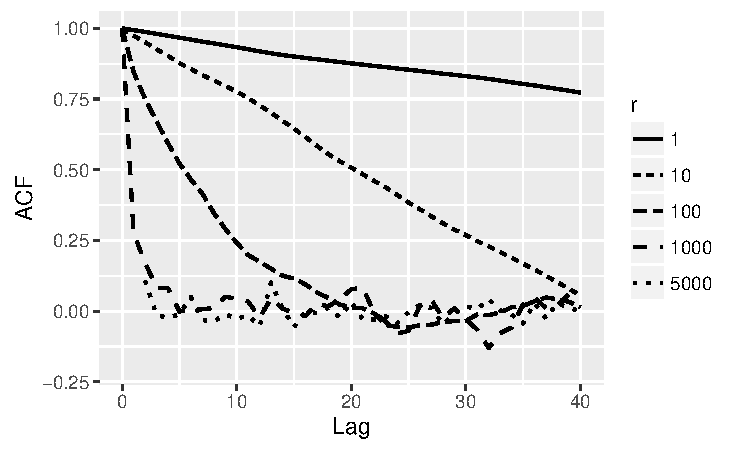
\includegraphics[width=1\textwidth]{probit_demo_acf_prop.pdf}
  \caption{ACF for CDA without M-H adjustment.}
 \label{probit_demo_intercept_proposal}
\end{subfigure}
  \hfill
    \begin{subfigure}[b]{0.32\textwidth}
 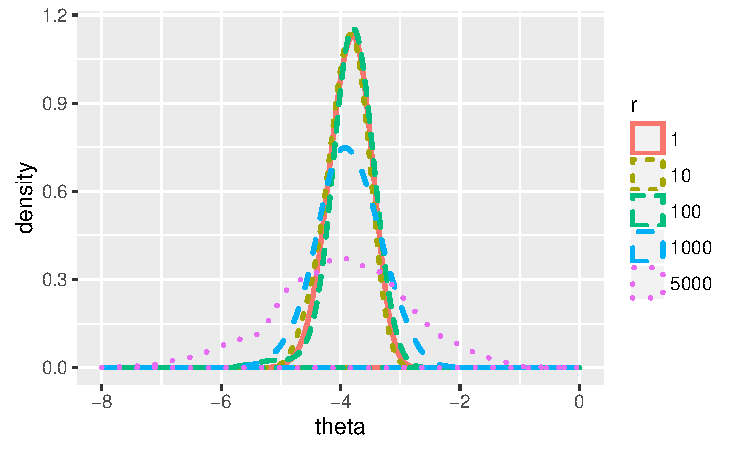
\includegraphics[width=1\textwidth]{density_probit.pdf}
  \caption{Density estimates of the posterior without M-H adjustment.}
   \label{probit_demo_intercept_density}
\end{subfigure}
\hfill
   \begin{subfigure}[b]{0.32\textwidth}
 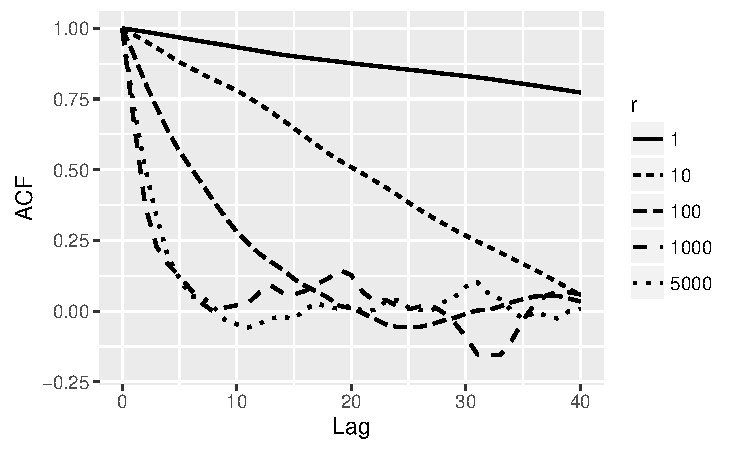
\includegraphics[width=1\textwidth]{probit_demo_acf.pdf}
  \caption{ACF for CDA with M-H adjustment}
   \label{probit_demo_intercept_posteriorsample}
\end{subfigure}
  \hfill
  \caption{ Autocorrelation functions (ACFs) and kernel-smoothed density estimates for different CDA samplers in intercept-only probit model.}
 \label{probit_demo_intercept}
 \end{figure}


\subsection{Choice of calibration parameters} %using Asymptotic Approximation}

As illustrated in the previous subsection, efficiency of CDA is dependent on a good choice of the calibration parameters $r=(r_1,\ldots,r_n)$ and $b=(b_1,\ldots,b_n)$.  In this subsection, we propose a simple and efficient algorithm for calculating these parameters relying on Fisher information.  We will describe this algorithm in the probit case, but it is straightforward to apply much more broadly.  Letting the linear predictor in the probit model be denoted $\eta_i = x_i\theta$, the Fisher information based on the marginal and the conditional posteriors are:
\be
X' \diag\bigg\{\frac{\phi(\eta_i)^2}{ {\Phi(\eta_i)(1- \Phi(\eta_i))}}\bigg\} X,\quad \quad X' R^{-1} X
\ee
respectively, where $\phi$ is the standard normal density. Therefore, setting $r_i = \frac{\Phi(\eta_i)(1- \Phi(\eta_i))} {\phi(\eta_i)^2}$ completely adjusts for mis-calibration.  The $r_i$'s can be calculated using this expression quickly and easily without need to calculate the information matrix.
The bias-adjustment parameters $b$ are then chosen to increase the acceptance rate in the M-H step, $1\wedge \prod_i \frac{   L_r(\eta_i;y_i) L(\eta_i^*;y_i)}{ L_r(\eta_i^*;y_i)L(\eta_i;y_i) }$. In particular, by setting $b_i = \eta_i (\sqrt{r_i}-1)$ we ensure that $L_r(\eta_i;y_i) = L(\eta_i;y_i)$.
% LEO - CAN WE ACTUALLY CHOOSE b_i's to technically maximize the acceptance rate.  This is a bit squishy as is.

Since $\theta$ and $\eta$ are not known before sampling, we use a short tuning period to sample them and update $r$ and $b$ at the end of each iteration.  After tuning, we stop adaptation and keep $r$ and $b$ fixed.  To illustrate, we consider a probit regression with an intercept and two predictors $x_{i,1},x_{i,2}\sim \No(1,1)$, with $\theta=(-5,1,-1)'$, generating $\sum y_i=20$ among $n=10,000$. The \cite{albert1993bayesian} DA algorithm mixes slowly (Figure~\ref{probit_reg_trace} and \ref{probit_reg_acf}). We also show the 
results of the parameter expansion algorithm (PX-DA) proposed by \cite{liu1999parameter}. PX-DA only mildly reduces the correlation, as it does not solve the variance mismatch problem.  In contrast, applying CDA after a tuning period of 100 iterations, we obtain dramatically better mixing.

%We started CDA with the adaptive algorithm for 100 iterations, obtaining an acceptance rate of $0.43$, then ran $100$ steps as burn-in and collected the posterior sample for $500$ steps. 

 
\begin{figure}[H]
 % \centering
  \begin{subfigure}[b]{0.45\textwidth}
 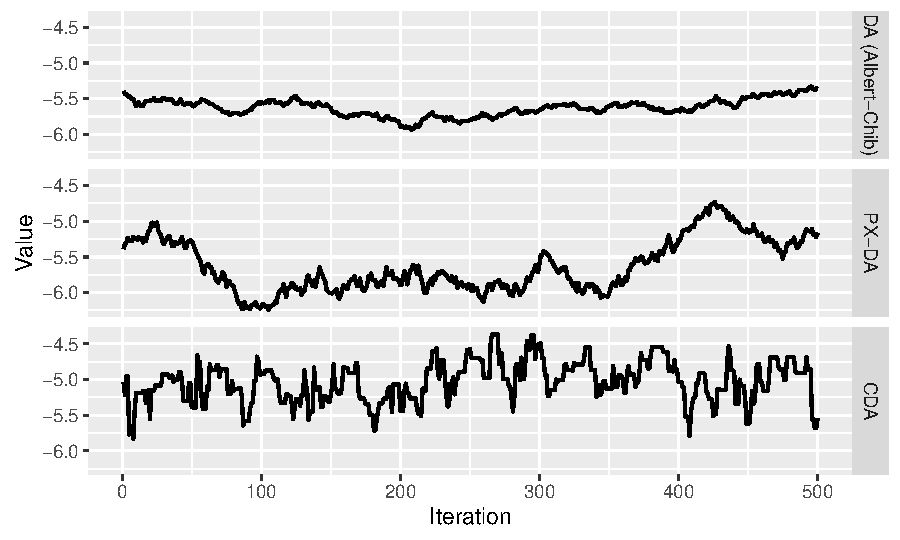
\includegraphics[width=1\textwidth]{probit15_trace_plot.pdf}
  \caption{Traceplot for the original DA, parameter expanded DA and CDA algorithms.}
  \label{probit_reg_trace}
\end{subfigure}
  \hfill
   \begin{subfigure}[b]{0.45\textwidth}
 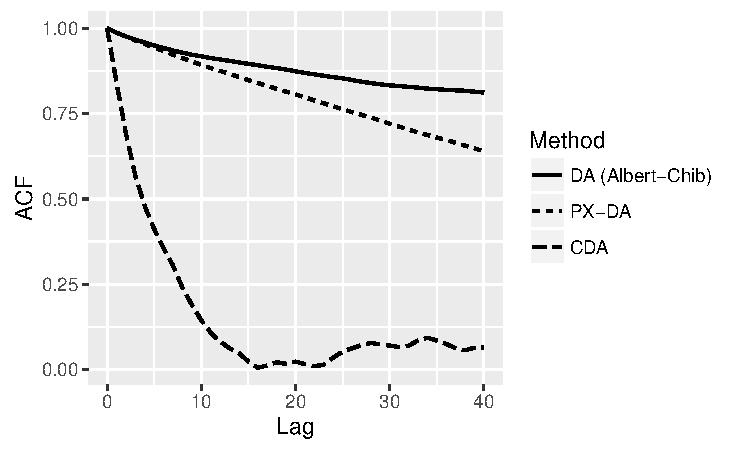
\includegraphics[width=1\textwidth]{probit15_acf.pdf}
  \caption{ACF for original DA, parameter expanded DA and CDA algorithms.}
    \label{probit_reg_acf}
\end{subfigure}
 \caption{Panel (a) demonstrates in traceplot and panel (b) in autocorrelation the substantial improvement in CDA by correcting the variance mis-match in probit regression with rare event data, compared with the original \citep{albert1993bayesian} and parameter-expanded methods \citep{liu1999parameter}.}
 \end{figure}

\subsection{Logistic regression example: A second calibration approach}

Calibration was easy to achieve in the probit examples, because $\mbox{var}( \theta | z,y)$ does not involve the latent variable $z$.  In cases in which the latent variable impacts the variance of the conditional posterior distribution of $\theta$, we propose a different calibration strategy based on inflating the variance of $\pi(z|y)$ targeted towards increasing 
$\bb E_z \mbox{var}(\theta|z,y)$.  In developing this second calibration strategy, we focus on the logistic regression model with 
\be
y_i \sim \Bern(p_i), \quad p_i = \frac{\exp(x_i \theta)}{1+\exp(x_i \theta)},
\ee
and improper prior $\pi(\theta)=1$. For this model, \cite{polson2013bayesian} proposed Polya-Gamma data augmentation:
\be
 z_i &\sim {\PG}(1, |\xbeta|),\\
\theta &\sim \No \left(  (X' Z X)^{-1}   X'  (y-0.5)  ,  (X' Z X)^{-1}  \right),
\ee
where $Z= \diag(z_1,\ldots,z_n)$.  This algorithm relies on expressing the logistic regression likelihood as
$$L(y_i \mid \xbeta)=  \int \exp\{ \xbeta (y_i-1/2)\} \exp\bigg\{ -\frac{z_i (\xbeta)^2}{2}\bigg\} \PG(z_i \mid 1,0) dz_i,$$
where $\mbox{PG}(a_1,a_2)$ denote the Polya-Gamma distribution with parameters $a_1,a_2$, with $\bb{E}z_i= \frac{a_1}{2 a_2}\tanh(\frac{a_2}{2})$.
%As described above, multiplying $r_i$ on $z_i$ is ineffective and makes the integration intractable.

Our previous calibration approach would have relied on inflating the variance in the conditional update of $\theta$, but this unfortunately no longer works well due to the occurence of $Z$ in the conditional covariance.  Instead, we rely on replacing $\PG(z_i \mid 1,0)$ with $\PG(z_i \mid r_i,0)$ in the step for updating the latent data.  Smaller $r_i$ can lead to larger  $\bb E_z \mbox{var}(\theta|z,y)$, providing a route towards calibration.  Applying the bias-adjustment term $b_i$ to the linear predictor $\eta_i = x_i\theta$ leads to 
\be
L_r(\xbeta;y_i) = & \int_{0}^{\infty}  \exp\{ (\xbeta+b_i) (y_i-r_i/2)\} \exp\bigg\{ -\frac{z_i (\xbeta+b_i)^2}{2}\bigg\} \PG(z_i \mid r_i,0) dz_i \\
= &  \frac{\exp \{ (x_i \theta + b_i)y_i \}}{\{1+\exp(\xbeta +b_i)\}^{r_i}},
\label{eq:prop-marginal-logit}
\ee
and the update rule for the proposal:
\be
 z_i &\sim {\PG}(r_i, |\xbeta+b_i|),\\
\theta^* &\sim \No \left(  (X' Z X)^{-1}  X'  (y -r/2- Zb) ,  (X' Z X)^{-1}  \right),
\ee
with acceptance probability:
\be
1 \wedge  \frac{  \prod_i L_r(\xbeta;y_i) L(\xbeta^*;y_i)}{\prod_i  L_r(\xbeta^*;y_i)L(\xbeta;y_i) } =1 \wedge \prod_i  \frac{ \{1+\exp(\xbeta)\}   \{1+\exp(\xbeta^*+b_i)\}^{r_i} } {  \{1+\exp(\xbeta^*)\}  \{1+\exp(\xbeta+b_i)\}^{r_i}    },
\ee
where $L(\theta;y_i)=\frac{\exp(\theta y_i)}{1+\exp(\theta)}$.

To demonstrate why smaller $r_i$ leads to larger $\bb E_z (X' Z X)^{-1}$, we compute the  first negative moment of the Polya-Gamma distribution. Combining \cite{cressie1981moment} and \cite{polson2013bayesian}, $\bb{E}z_i^{-1}= \int_0^{\infty} \prod_{k=1}^{\infty} (1+ d_k^{-1} t) ^{-r_i} dt$ with $d_k=2(k-\frac{1}{2})^2\pi^2 + \frac{(x_i\theta+b_i)^2}{2}$.

For choosing $r$ during tuning, we compare the two Fisher information matrices based on the marginal and conditional; for the latter, we marginalize out $z_i$ by taking the expectation:
\be
X' \diag\bigg\{\frac{\exp(\xbeta)}{ \{1+\exp(\xbeta)\} ^2}\bigg\} X, \quad X'  \diag\bigg\{ \frac{r_i}{2 |\xbeta+b_i|}\tanh\Big(\frac{|\xbeta+b_i|}{2} \Big)\bigg\} X
\ee
To correct the difference, we choose $r_i$ to be $\frac{\exp(\xbeta)}{ \{1+\exp(\xbeta)\} ^2} {2 |\xbeta+b_i|}/ \tanh(\frac{|\xbeta+b_i|}{2})$. To optimize the acceptance rate, given the value of $r_i$ and $\xbeta$,  setting $ \{1+\exp(\xbeta)\}  = \{1+\exp(\xbeta+b_i)\}^{r_i}  $ yields $b_i = \log[  \{1+\exp(\xbeta)\}^{1/r_i} -1] - \xbeta$.


As a numerical illustration, we use a two parameter intercept-slope model with $x_1\sim \No(0,1)$ and $\theta=(-9,1)'$. With $n= 10^5$, we obtain rare outcome data with 
 $\sum y_{i} = 50 $.  We ran the original DA algorithm  \citep{polson2013bayesian} and an independence chain M-H sampler using a multivariate normal proposal $\theta^*|\theta \sim \No(\theta^*| \theta, {\mc I}^{-1}(\theta))$, with ${\mc I}(\theta)$ the Fisher information matrix based on the marginal posterior. For CDA we tuned $r$ and $b$ for $100$ steps, reaching an acceptance rate of $0.8$, and then stopped adaptation and ran an additional burn-in of 100 iterations, with the following 500 samples collected.  Shown in Figure~\ref{logit_random_mixing}, both DA and M-H with a normal proposal mix slowly, exhibiting strong autocorrelation even lag $40$, while CDA has dramatically better mixing.

\begin{figure}[H]
 % \centering
  \begin{subfigure}[b]{0.49\textwidth}
 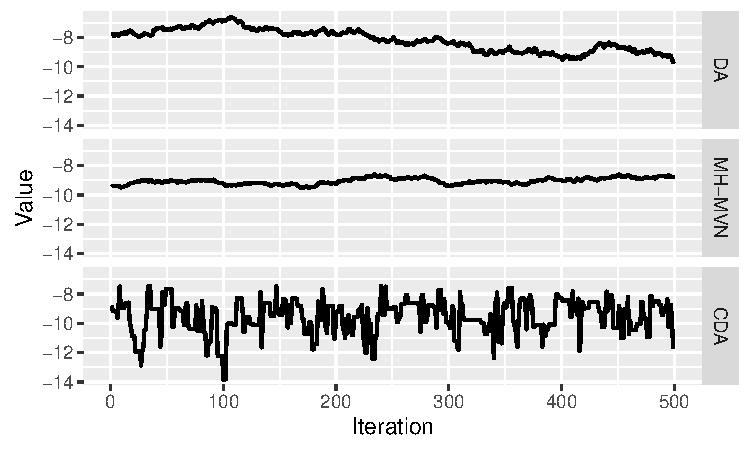
\includegraphics[width=1\textwidth]{logit_demo_trace_plot}
  \caption{Traceplots for DA, CDA and M-H with multivariate normal proposal.}
\end{subfigure}
  \hfill
   \begin{subfigure}[b]{0.49\textwidth}
 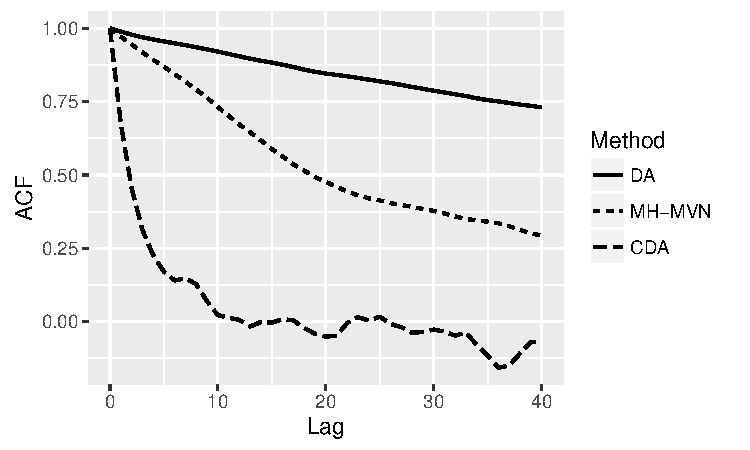
\includegraphics[width=1\textwidth]{logit_demo_acf}
  \caption{ACF for DA, CDA and M-H with multivariate normal proposal.}
\end{subfigure}
 \caption{Panel (a) demonstrates in traceplot and panel (b) in autocorrelation the substantial improvement of CDA in logistic regression with rare event data, compared with the original DA \citep{polson2013bayesian} and the M-H algorithm with multivariate normal proposal (MH-MVN).}
    \label{logit_random_mixing}
 \end{figure}

\subsection{General Algorithm}

Before providing theoretical support for CDA, we summarize the algorithm in more generality, noting that substantial further generalizations are possible (e.g., to accommodate hierarchical, temporal and spatial dependence).  We assume the parameters are multi-dimensional and can be divided into two groups $\{ \theta, \tau\}$, with $\theta$ and $\tau$ sampled separately based on their conditional posterior distributions.  For notational ease, we focus on $\theta$ and omit the conditioning on $\tau$ in the rest of the subsection.  Assume $\theta$ can be augmented with latent variable $z$ but is susceptible to slow mixing. The augmented likelihood can be expressed as 
\be \label{eq:da_decomposition}
\prod_i L(m_i(\theta);y_i) =\prod_i   \int \pi\left(m_i(\theta)|z_i,y_i \right)\pi(z_i|y_i) d z_i,
\ee
where  $m_i(\theta)$ is a continuous and differentiable function $m_i:\bb R^p \mapsto \bb R^d$. For example,  $m_i (\theta) = x_i\theta$ is the linear predictor in regression. Let
the conditional distribution for $z$ and $\theta$ be, respectively,
\be
z_i \mid \theta, y &\sim \pi (z_i; m_i(\theta), y)\\
\theta \mid z,y &\sim f( \theta; \mu,\Sigma),
\ee
where $f( \theta; \mu,\Sigma)\propto \pi(\theta) \prod_i \pi\left(m_i(\theta)|z_i,y_i \right)$. To calibrate the variance $\Sigma$, we introduce a parameter $r_i$. When $\Sigma$ is free from $z$, we put $r_i$ in each $\pi\left(m_i(\theta)|z_i,y_i \right)$ as in the probit examples above. When $\Sigma$ involves $z$, we put $r_i$ in $\pi(z_i|y_i)$ to increase $\bb E_z\Sigma$ as in the logit examples. Then using another parameter $b_i$ to accommodate the shift in $m_i(\theta)$, we obtain the calibrated data augmentation:
\be \label{eq:cda_decomposition}
\prod_i L_r(m_i(\theta) ; y_i,  r_i, b_i) = \prod_i \int \pi_r\left(m_i(\theta)+b_i|z_i,y_i \right)\pi_r(z_i|y_i) d z_i.
\ee
With prior $\pi(\theta)$, the proposal can then be sampled from the calibrated distribution:
\be
z_i & \sim \pi_r(z_i; m_i(\theta)+b_i, y) \\
\theta^* &\sim f( \theta^*|\mu(r, b),\Sigma(r)).
\ee
in an M-H step with acceptance probability:
\be
1 \wedge \prod_i  \frac{L(m_i(\theta^*); y_i) L_r(m_i(\theta) ; y_i)} {L(m_i(\theta); y_i, r_i, b_i) L_r(m_i(\theta^*); y_i, r_i, b_i)}.
\label{eq:mh-criterion}
\ee
In an initial tuning phase, we adaptively update $r$ and $b$. We choose $r$ at each sampling step to minimize the difference between the Fisher information matrices based on the marginal posterior with the latent data integrated out and the conditional posterior given the latent data.  As illustrated in subsection 2.3-2.4 for the two different strategies of augmentation, simple and computationally efficient closed forms are typically available for the $r_i$'s, which avoid potentially expensive calculation of the full information matrix.
Then conditional on $r_i$, we choose $b_i$ to increase the M-H acceptance rate; one choice is the solution to $L_r(m_i(\theta); y_i,  r_i, b_i)=L(m_i(\theta); y_i)$. 

\section{Theory: Mixing Acceleration}

We studying the theory behind the acceleration of mixing after calibration focusing on samples collected for fixed values of $r,b$ after the adaptation period.
The mixing rate of a Markov chain can be described by the geometric convergence rate. Let $\mathcal{P}(\theta,.)$ be the Markov transition measure, $\pi(.)$ be the target invariant measure and $\theta$ be the state in the state space $\varTheta$. Starting from the initial state $\theta^{(0)}$, the chain is geometrically ergodic if there exist $M: \varTheta \rightarrow [0, \infty)$ and $\rho\in[0,1)$ such that $||\mathcal{P}^k(\theta,.)-\pi(.) ||_{TV} \le M(\theta^{(0)}) \rho^k$, where $||.||_{TV}$ is the total variation distance $|| P_1 -P_2 ||_{TV} = \underset{\mathcal A\in \mathcal F}\sup ||P_1(\mathcal A)-P_2(\mathcal A)||$. As the number of iterations $k\rightarrow \infty$, $||\mathcal{P}^k(\theta,.)-\pi(.) ||_{TV} \rightarrow 0$ leading to convergence to the target. Slow mixing corresponds to $\rho$ being close to $1$. 
%As shown by \cite{scott2016bayes}, $\rho$ approaches $1$ as $n$ increases, leading to a complete break-down of algorithm.  {\bf THIS SEEMS THE WRONG CITE AND TOO GENERAL A STATEMENT}

We first utilize another related quantity, the norm of the forward operator $||\bf{F}||$, which is defined as  ${\bf F}s(\theta)=\int \mathcal{P}(\theta,\theta') s(\theta') d\theta' = E\{ s(\theta') | \theta \}$. In a Hilbert space $L^2(\pi)=\{s(\theta): \bb E s(\theta)=0, \mbox{var}\{s(\theta)\}<\infty \}$, the norm is defined as the maximal correlation between two states $||{\bf F}||=\underset{s(\theta),t(\theta)\in L^2(\pi)}{\sup}\;\mbox{corr}(s(\theta),t(\theta^{'}))$ \citep{liu2008monte}. This norm is related to $\rho$: when the chain is reversible with detailed balance (e.g. M-H), $\lim_{k\rightarrow \infty}||{\bf F}^k||^{1/k}=\rho$; when the chain is non-reversible, $||{\bf F}||^2$ is equal to the convergence rate of the reversibilized chain \citep{fill1991eigenvalue}.

In each iteration, Gibbs sampling sequentially update all the parameters $\theta$ and the latent variable $z$. We denote the last state as $z'$ and $\theta'$ and the new state as $z$ and $\theta$. Then the original DA sample in the order of $\theta' \rightarrow z' \rightarrow \theta \rightarrow z$, where $a\rightarrow b\rightarrow c$ means that given $b$, $c$ is conditionally independent of $a$.

In calculation, omitting the first and last steps do not alter the maximal autocorrelation (Lemma 4 in \cite{liu1994collapsed}), leading to:

\be
||{\bf F}_{DA}|| =\underset{s(\theta)\in L^2(\pi)}{\sup}\; \frac{\mbox{var}_{DA} [ \bb E_{DA} \{ s(\theta,z)|\theta^{'},z'\}]}{\mbox{var}_{DA}\{s(\theta,z) \} }  & = \underset{s(\theta)\in L^2(\pi)}{\sup}\; \frac{\mbox{var}_{DA} [ \bb E_{DA} \{ s(\theta)|z'\}]}{\mbox{var}_{DA}\{s(\theta) \} } \\
& = 1- \underset{s(\theta)\in L^2(\pi)}{\inf}\; \frac{\bb E_{DA}  [  \mbox{var}_{DA}\{ s(\theta)|z'\}]}{\mbox{var}_{DA}\{s(\theta) \} } 
\label{eq:norm_da}
\ee
where the last form without the infimum is known as Bayesian fraction of missing information \citep{papaspiliopoulos2007general}. Slow mixing occurs when ${\bb E_{DA}  [  \mbox{var}_{DA}\{ s(\theta)|z'\}]} \ll {\mbox{var}_{DA}\{s(\theta) \} }$.

Calibrated DA samples a little differently: by proposing $\theta^*$ in the calibrated sample and using Metropolis-Hastings to accept the new state $\theta^*$ with probability $p(\theta^*,\theta')$ or keep the previous state $\theta$, it in fact samples from a two-component mixture:

\be
\theta  \sim (1-p(\theta^*,\theta') ) \delta _{\theta'} + p(\theta^*,\theta') f(\theta^*\mid z').
\ee

Therefore, the updating sequence is $\theta'\rightarrow z'$ and $(\theta', z')\rightarrow \theta \rightarrow z$. Similarly, omitting the last step of updating $z$ does not alter the maximal autocorrelation, leading to:

\be
||{\bf F}_{CDA}|| =\underset{s(\theta)\in L^2(\pi)}{\sup}\; \frac{\mbox{var}_{CDA} [ \bb E_{CDA} \{ s(\theta,z)|\theta^{'},z'\}]}{\mbox{var}_{CDA}\{s(\theta,z) \} }  = 1- \underset{s(\theta)\in L^2(\pi)}{\inf}\; \frac{\bb E _{CDA} [  \mbox{var}_{CDA}\{ s(\theta)|z',\theta'\}]}{\mbox{var}_{CDA}\{s(\theta) \} } 
\label{eq:norm_cda}
\ee


To compare the \eqref{eq:norm_da} and \eqref{eq:norm_cda} directly, we rely on the following lemma.

\begin{lemma}
	In Metropolis-Hastings step with current state $\theta'$ and proposal state $\theta^*$ from $f(\theta^*; z')$, if the acceptance probability $p\ge p_0$, the generated state $\theta$ satisfies $\mbox{var}_{CDA}\{ s(\theta)|z', \theta'\} \ge   p_0\cdot \mbox{var}_{CDA} (s(\theta^*)|z')$.
\end{lemma}

Therefore, for a given $s(\theta)$, we can induce an increase in $\bb E [\mbox{var}\{ s(\theta')|z'\}]$ by $\gamma$ times over $\bb E [\mbox{var}\{ s(\theta)|z'\}]$, and obtain the following acceleration:

\begin{theorem}
Let ${\bf F}_{DA}$ and ${\bf F}_{CDA}$ be the forward operators corresponding to the standard DA and the calibrated DA; $\theta$ be the random variable from the DA updating rule and $\theta^*$ be the one from the CDA proposal. Assume the conditional variance increase in the CDA proposal has ${  \bb E [\mbox {var}_{CDA}\{ s(\theta^*)|z,y\}]  } \ge \gamma \cdot { \bb E [\mbox {var}_{DA}\{ s(\theta)|z,y\}]}$ with the Metropolis-Hastings acceptance probability in \eqref{eq:mh-criterion} greater or equal to $p_0>0$. Then if $p_0 \gamma \ge 1$, 
$$||{\bf F}_{CDA}||\le 1- \gamma p_0 \cdot \underset{s(\theta)\in L^2(\pi)}{\inf}\; \frac{\bb E_{DA}  [  \mbox{var}_{DA}\{ s(\theta)|z'\}]}{\mbox{var}_{DA}\{s(\theta) \} } 
\le ||{\bf F}_{DA}||.$$
\end{theorem}

It is often not tractable to examine every $s(\theta)\in L^2(\pi)$; but in practice, it suffices to check $s(\theta)=\theta_j$ for every element in $\theta$ \citep{yang2013sequential}. Therefore, the ideal $r_i$ would be close to $\frac{\mbox{var}_{DA}\{\theta \} } {\bb E_{DA}  [  \mbox{var}_{DA}\{ \theta|z'\}]}$ so that $||{\bf F}_{CDA}||\approx 1 - p_0$. Both the numerator and the denominator often lack closed-forms for finite sample, but can be approximately estimated with a term proportional to the Fisher information. As the result, . In our study cases, all of the CDA's have large $p_0$, which is attributed to the distributional similarity between $L_r$ and $L$ in \eqref{eq:mh-criterion}.


\section{Co-Browsing Behavior Application}

We apply CDA to an online browsing activity dataset. The dataset contains a two-way  table of visit count by users who browsed one of $96$ client websites of interests, and one of the  $n=59,792$ high-traffic sites during the same browsing session. We refer to visiting more than one site during the same session as co-browsing. For each of the client websites, it is of large commercial interests find out the high-traffic sites with relatively high co-browsing rates, so that ads can be more effectively placed. For the computational advertising company, it is also useful understand the the co-browsing behavior and predict traffic pattern of users. We consider two models for these data.


\subsection{Hierarchical Binomial Model for Estimating Co-browsing Rates}

We initially focus on one client website and analyze co-browsing rates with the high-traffic sites. With the total visit count $N_i$ available for the $i$th high-traffic site, the count of co-browsing $y_i$ can be considered as the result of a binomial trial. with $y_i$ extremely small relative to $N_i$ (with ratio  ($0.00011 \pm  0.00093$)), the maximum likelihood estimate $y_i/N_i$ can have poor performance. For example, when $y_i=0$, estimating the rate as exactly $0$ is not ideal. Therefore, it is useful to consider a hierarchical model to allow borrowing of information across high-traffic sites.

\be
y_i \sim \Binom\left(N_i, \frac{\exp(\theta_i)}{1+\exp(\theta_i)}\right), \quad \theta_i\stackrel{iid}{\sim} \No(\theta_0, \sigma^2_0), \quad i=1\ldots n\\
(\theta_0,\sigma^2_0) \sim  \pi(\theta_0,\sigma^2_0) 
\ee
Based on expert opinion in quantitative advertising, we use a weakly informative prior $\theta_0\sim \No(-12,49)$ and uniform prior on $\sigma^2_0$. Similar to the logistic regression, we calibrate the binomial Polya-Gamma augmentation, leading to the proposal likelihood:

\be
L_r(\theta_i: y_i,N_i, r_i, b_i) = \frac{\exp(\theta_i+b_i)^y_i}{\{ 1+\exp(\theta_i+b_i)\}^{N_ir_i}}
\ee

Conditioned on the latent Polya-Gamma latent variable $z_i$, each proposal $\theta^*_i$ can be sampled from:

\be
z_i &\sim \PG\left ( (N_ir_i),\theta_i+b_i \right)\\
\theta_i^* &\sim \No \left( \frac{ y_i - r_i N_i/2 -z_i b_i + \theta_0/\sigma^2_0}{z_i+ 1/\sigma^2_0}, \frac{1}{z_i+ 1/\sigma^2_0}\right),
\ee
and accepted or rejected using an M-H step. Similar to logistic regression, the auxiliary parameters are chosen as $r_i =\frac{\exp(\theta_i)}{ \{1+\exp(\theta_i)\} ^2} {2 |\theta_i+b_i|}/ \tanh(\frac{|\theta_i+b_i|}{2})$ and $b_i=\log[  \{1+\exp(\theta_i)\}^{1/r_i} -1] - \theta_i$ during adaptation. Since $\theta_i$'s are conditionally independent, the calibrated proposal can be individually accepted with high probability for each $i$. This leads to a high average acceptance of $0.9$, despite the high dimensionality of $59,792$ $\theta_i$'s.

Figure~\ref{data_binomial} shows the boxplots of the ACFs for all $\theta_i$'s. We compare the result with the original DA \citep{polson2013bayesian}. We run each algorithm for $4,000$ steps and use the last $1,000$ as the posterior sample. All of the parameters mix poorly in DA; CDA leads to significant improvement with autocorrelation rapidly decaying to close to zero within $5$ lags. Table~\ref{tab:binomial} lists the posterior mean and standard deviation for $\theta_0$ and $\sigma_0^2$, as well as the computing time per every $1,000$ steps. To provide a reference, we ran Hamiltonian Monte Carlo (HMC) provided by the Stan software \citep{carpenter2016stan}. HMC enjoys good mixing performance but is computationally intensive due to the numeric leapfrog steps. The parameter estimates from CDA and HMC are remarkably close, while critically slow mixing in the original DA caused poor estimates.


 \begin{figure}[H]
 % \centering
   \begin{subfigure}[b]{0.45\textwidth}
 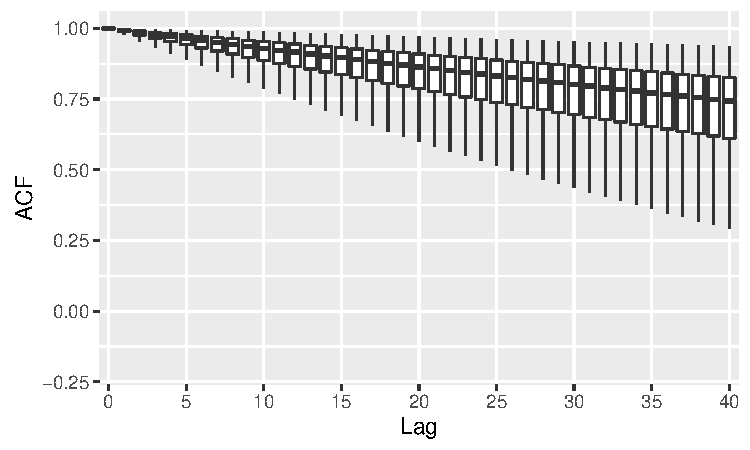
\includegraphics[width=1\textwidth]{binomial_random_acf_da.pdf}
 \caption{ACFs of the rate parameters $\theta_i$ using DA.}
 \end{subfigure}
  \hfill 
 \begin{subfigure}[b]{0.45\textwidth}
 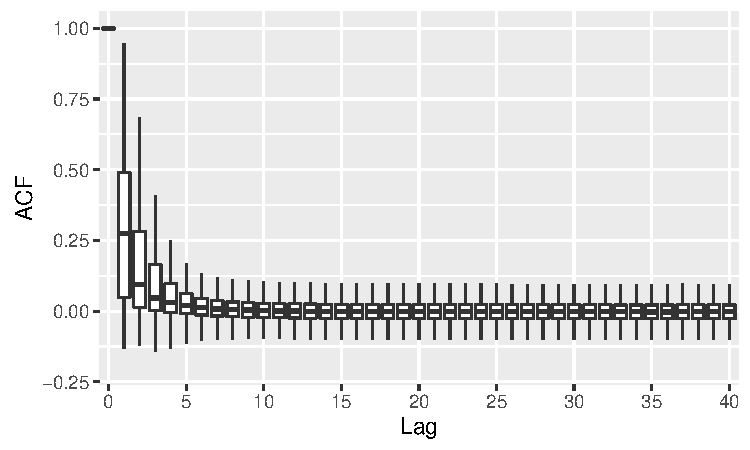
\includegraphics[width=1\textwidth]{binomial_random_acf_cda.pdf}
 \caption{ACFs of the rate parameters $\theta_i$ using CDA.}
 \end{subfigure} 
 \caption{Boxplots of the ACFs show the mixing of the $59,792$ parameters in the hierarchical binomial model, for the original DA\citep{polson2013bayesian} and CDA.}
 \label{data_binomial}
 \end{figure}
 
 
 
\begin{table}[H]
\centering
\begin{tabular}{|l |r |r| r| r |} 
 \hline
                          & DA & CDA & HMC\\
 [0.5ex]
 \hline
$\theta_0$                         & -9.33 (0.12)& -12.05 (0.02) &  -12.01 (0.02)\\
$\sigma^2$         & 0.76 (0.10)&   7.70 (0.10)  & 7.67 (0.10)\\
Computing Time (per 1,000 steps)  & 20 mins       & 20 mins        & 200 mins\\
 \hline
\end{tabular}
\caption{Parameter estimates and computing speed of the DA, CDA and HMC in hierarchical binomial model. CDA provides parameter estimates as accurate as HMC, while adds almost no computational cost based on DA.}
\label{tab:binomial}
\end{table}


\subsection{Poisson Regression for Web Traffic Prediction}

We now focus on a slightly different problem: it is useful to predict the traffic to one client website, using the information from the other $95$. Therefore, we consider a Poisson regression model with random effects:

\be
y_i \sim \Poi\left( \tau_i \exp  (\xbeta )\right),  \quad \tau_i\stackrel{iid}{\sim} \Ga(1, 1), \quad i=1\ldots n\\
\theta \sim  \No(0,\Sigma).
\ee

Since the dimensionality of the fixed effect random parameters $\theta$ is moderately large ($96$ with the intercept), we assign a diffuse prior with $\Sigma= I\cdot 100$. To allow over-dispersion, we use a gamma prior for $\tau_i$ with prior mean $1$, and the random effect can be sampled from $\tau_i \sim \Ga\left(1+y_i, 1+\exp(\xbeta) \right)$. As an alternative, one can assign normal random effect $\log \tau_i \sim N(0,\sigma^2_0)$ and use CDA to sample its posterior given $\xbeta$, similar to the binomial example. For simplicity, we choose Gamma prior for $\tau$ for its closed-form posterior.

The data augmentation for Poisson log-normal model is much less known. \cite{zhou2012lognormal} proposed to utilize a limit form. We present a simplified form:

\be
L(\xbeta,\tau_i;y)=\frac{\tau_i^{y_i}}{ y!}\frac{ \exp(y_i \xbeta) }{\exp\{\tau_i\exp(\xbeta)\}} =\frac{\tau_i^{y_i}}{ y!} \lim_{\lambda\rightarrow\infty}\frac{\exp(y_i \xbeta)}{\{1+ \exp(\xbeta + \log \tau_i)/\lambda\}^{\lambda}}.
\ee

\cite{zhou2012lognormal} used a moderate $\lambda=1,000$ to approximate the likelihood, hence enabled a Polya-Gamma augmented sampling:

\be
z_i \sim & \PG\left (\lambda, \xbeta + \log \tau_i-\log \lambda\right)\\
\theta \sim & \No \left( \big[ (X' Z X+  0.01 \cdot I )^{-1}  X'  \big ( y - \lambda/2 - z (\log \tau_i-\log \lambda)\big) ,(X' Z X+  0.01 \cdot I )^{-1} \right)
\ee

 However, this augmentation has a critical issue: we discover that $\lambda$ needs to be much larger to ensure low approximation error. With $\eta_i=\xbeta + \log\tau_i$, the log of the denominator on the right hand side has $\lambda\log(1+\exp\left(\eta_i)/\lambda\right)= \exp(\eta_i) + \bigO(\exp(2\eta_i)/\lambda)$, hence $\lambda$ needs to be around $10^9$ to accommodate moderately large $\eta_i \approx 10$. On the other hand, large $\lambda$ would lead to extremely large $z_i$ and hence very slow mixing.

Using the calibration on the Polya-Gamma augmentation, we obtain the calibrated proposal likelihood:

\be
L_r(\xbeta;y_i)=\frac{\exp(\xbeta  +\log \tau_i -\log \lambda +b_i)^{y_i}}{\{1+ \exp(\xbeta + \log \tau_i -\log \lambda +b_i)\}^{\lambda r_i}},
\ee
and update rule:

\be
z_i \sim & \PG\left (\lambda r_i, \xbeta + \log \tau_i-\log \lambda+b_i\right)\\
\theta^{*} \sim & \No \left( \big[ (X' Z X+  0.01 \cdot I )^{-1}  X'  \big ( y - \lambda r/2 - z (\log \tau_i-\log \lambda + b)\big) ,(X' Z X+  0.01 \cdot I )^{-1} \right),
\ee
with acceptance probability.
\be
1 \wedge \prod_i  \frac{ \exp \{ \tau_i\exp (\xbeta)\}}{ \exp \{ \tau_i\exp (\xbeta^*)\}} \frac {{\{1+ \exp(\xbeta^{*} + \log \tau_i -\log \lambda +b_i)\}^{\lambda r_i}}}{{\{1+ \exp(\xbeta + \log \tau_i -\log \lambda +b_i)\}^{\lambda r_i}}},
\ee
which is based on the exact Poisson log-normal density.

To compare the mixing performance, we run the approximate DA with supposedly efficient albeit inaccurate $\lambda=1,000$, the CDA with $\lambda=10^9$ in the M-H proposal and the HMC. We ran each algorithm for $4,000$ steps and use the last $1,000$ as the posterior sample. For CDA, we used the first $1,000$ steps for adaptating $r$ and $b$, and obtained an acceptance rate of $0.6$. Figure~\ref{data_poisson} shows the mixings of DA and CDA. Even with relatively moderate $\lambda$, the DA still shows very slow mixing that all of the parameters mixes poorly; the CDA substantially improves the mixing.

 \begin{figure}[H]
 % \centering
  \begin{subfigure}[b]{0.45\textwidth}
 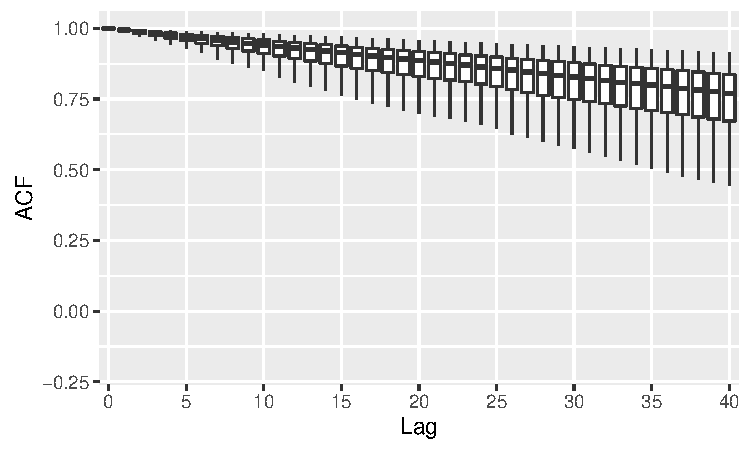
\includegraphics[width=1\textwidth]{poisson_acf_da}
 \caption{Autocorrelation of the parameters from DA.}
 \end{subfigure}
  \hfill 
 \begin{subfigure}[b]{0.45\textwidth}
 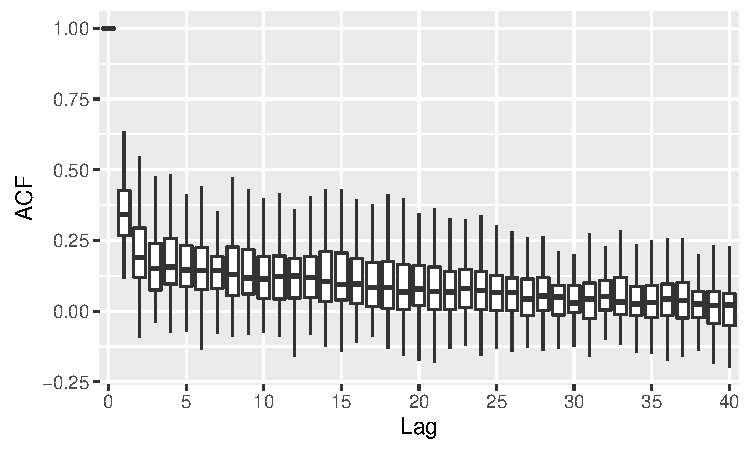
\includegraphics[width=1\textwidth]{poisson_acf_cda}
 \caption{Autocorrelation of the parameters from CDA.}
 \end{subfigure}
 \caption{CDA significantly improves the mixing of the parameters in the Poisson log-normal.}
 \label{data_poisson}
 \end{figure}

Table~\ref{table:Poisson} lists the comparison for all three models. We include the posterior mean and standard deviation of the $1$-norm of the coefficients $\sum_{j=0}^{95} |\theta_j|$. For goodness-of-fit, we compute the root-mean-squared error $\text{RMSE}= \sqrt{ \sum_{i=1}^n  (y_i-\hat\tau_i\exp( x_i{\hat\theta}))^2/n}$ with ${\hat\theta}$ and $\hat\tau$ as the posterior mean. To evaluate the prediction performance, we use another validation dataset and $\hat y_{i,new}=\hat\tau_i\exp( x_{i,new}{\hat\theta})$ as the predictor. We evaluate the cross-validation RMSE between $y_{i,new}$ and $\hat y_{i,new}$. CDA and HMC perform quite well and the validation error that is $4$ times lower than DA. Like the binomial application, the CDA is almost 10 times faster than HMC.


\begin{table}[H]
\centering
\begin{tabular}{|l |r |r| r| r |} 
 \hline
                          & DA & CDA & HMC\\
 [0.5ex]
 \hline
$\sum_{j=0}^{95} |\theta_j|$         & 11.53 (0.10)&  7.42 (0.11)  & 7.51 (0.11)  \\
RMSE                              & 30.83        & 4.03          & 4.38\\
DIC                                 & $-4.1131 \times 10^5$     & $-5.1953 \times 10^5$      & $-5.1954 \times 10^5$\\
CV-RMSE                           & 33.21        & 8.52          & 8.18\\
Computing Time (per 1,000 steps)  & 25 mins       & 26 mins        & 300 mins\\
 \hline
\end{tabular}
\caption{Parameter estimates and computing speed of the DA, CDA and HMC in Poisson regression model. CDA shows similar performance as HMC in both parameter estimation and cross-validation in prediction, but is about 10 times faster.}
\label{table:Poisson}
\end{table}

\section{Discussion}

In posterior sampling, when the parameters lack closed-form in the marginal distribution, data augmentation is a useful technique. It has been realized that this practice could severely stall the mixing, due to the gap between the conditional variance with the augmented data and the marginal one. With data size increases and become complex, it is common for the conditional distribution of the parameter to deviate from the area that has reasonable mixing performance. As we show in the previous examples, this quickly leads to an un-manageable increase in the computational time and poor estimation.

To solve this problem, we propose a general class of method to calibrate the variance conditional on the latent variable. With a mechanism to adjust the step size, the transition in each iteration is corrected onto the same order of the marginal variance. The generated samples are used as proposal in the Metropolis-Hastings for exact posterior. In this article, we demonstrate that this strategy is applicable when $\theta \mid z$ belongs to the location-scale family. We expect that it can be extensible to any distribution with a variance / scale, possibly with a different bias-reducing mechanism.

There is some similarity between CDA and HMC. Both algorithms excel in seeking proposal with high acceptance rate. The difference is that quite often, the Hamiltonian lacks closed-form solution, and requires multiple steps numeric evaluations of the dynamics for one proposal; whereas CDA only needs one step. Therefore, when the data augmentation exists, CDA is always more efficient in computation.

In this article, we insist on obtaining the exact posterior, to provide an analysis on the mixing property. Without the Metropolis-Hastings step, the sampling strategy in calibrated data augmentation can be used alone to generate approximate posterior. This can be useful when the evaluation of the marginal likelihood is costly.

\bibliography{reference}
\bibliographystyle{plainnat}


\section{Appendix}

%
%\subsubsection{Proof of Theorem 1:}
%
%
%Let $\theta=\{\theta_1, \theta_2\}$ be the parameters that are divided into two parts. Let $\theta'$ and $z'$ be the parameters and latent variables in the last iteration. Omitting $y$ for the ease of notation, the square of maximal correlation can be represented as $||{\bf F}||^2=\underset{s(\theta,z),t(\theta,z)\in L^2(\pi)}{\sup}\;\mbox{corr}\{s(\theta,z),t(\theta^{'},z')\}^2
%= \underset{s(\theta,z)\in L^2(\pi)}{\sup}\; \frac{\mbox{var} [ E \{ s(\theta,z)|\theta^{'},z'\}]}{\mbox{var}\{s(\theta,z) \} }$.
%
%The original DA samples in the order of $ \{\theta'_1, \theta'_2\} \rightarrow z' \rightarrow \{\theta_1, \theta_2\}\rightarrow z$, with $ \mbox{var} [ E \{ s(\theta,z)|\theta^{'},z'\}] =  \mbox{var} [ E \{ s(\theta_1, \theta_2,z)|\theta^{'}_1,\theta^{'}_2,z'\}] $. The marginalization and sampling based CDA samples  in the order of $ \theta'_2 \rightarrow z' \rightarrow \theta_2\rightarrow z$, followed by $z' \rightarrow \theta'_1$ and  $z \rightarrow \theta_1$ with $ \mbox{var} [ E \{ s(\theta,z)|\theta^{'},z'\}] =  \mbox{var} [ E \{ s(\theta_1, \theta_2,z)|\theta^{'}_1,\theta^{'}_2,z'\}] = \mbox{var} [ E \{ s(\theta_1, \theta_2,z)|\theta^{'}_2,z'\}]$.
%
%For better clarity, let $E_{X}$ denote the integration over $P(dX)$. 
%
%\begin{equation}
%\begin{aligned}
% \mbox{var} [ E \{ s(\theta_1, \theta_2,z)|\theta^{'}_2,z'\}]  & = E_{\theta^{'}_2,z'}  [ E_{\theta_1, \theta_2,z}\{ s(\theta_1, \theta_2,z)|\theta^{'}_2,z' \} ]^2 -  (E_{\theta^{'}_2,z'}   [ E_{\theta_1, \theta_2,z}\{ s(\theta_1, \theta_2,z)|\theta^{'}_2,z' \} ])^2  \\
% & = E_{\theta^{'}_2,z'}   [ E_{\theta'_1}E_{\theta_1, \theta_2,z} \{ s(\theta_1, \theta_2,z)|\theta'_1, \theta^{'}_2,z' \} ]^2 - (E_{\theta^{'}_1,\theta^{'}_2,z'}   [ E_{\theta_1, \theta_2,z} \{ s(\theta_1, \theta_2,z)|\theta^{'}_1,\theta^{'}_2,z' \} ])^2 \\
%& \le  E_{\theta^{'}_2,z'}  E_{\theta'_1} [ E_{\theta_1, \theta_2,z} \{ s(\theta_1, \theta_2,z)|\theta'_1, \theta^{'}_2,z' \} ]^2 - (E_{\theta^{'}_1,\theta^{'}_2,z'}   [ E_{\theta_1, \theta_2,z} \{ s(\theta_1, \theta_2,z)|\theta^{'}_1,\theta^{'}_2,z' \} ])^2\\
%& =  \mbox{var}  [E \{ s(\theta_1, \theta_2,z)|\theta^{'}_1,\theta^{'}_2,z'\}] 
%\end{aligned}
%\end{equation}
%
%This completes the proof.


\subsection{Proofs}

\subsubsection{Lemma 1}
As the M-H step in CDA is equivalent to sampling from the mixture that:

\be
(1-p)\delta_{\theta'} + p f_{CDA}(\theta^*; z')
\ee
where $p$ is the acceptance probability in \eqref{eq:mh-criterion} and $f_{CDA}$ is the calibrated proposal distribution. Its conditional variance is:

\be
  \mbox{var}_{CDA}\{ s(\theta)|z', \theta'\} = & (1-p) s(\theta')^2 + p \bb E_{CDA} \{ s(\theta^*)^2|z'\}  - [ (1-p) s(\theta') + p \bb E_{CDA} \{ s(\theta^*)|z'\}]^2 \\
  = & (1-p) [s(\theta')^2 - (1-p) s(\theta')^2 - 2p s(\theta')  \bb E_{CDA} \{ s(\theta^*)|z'\}  + p \bb E_f \{ s(\theta^*)|z'\}^2 ] \\
  & + p [\bb E_{CDA} \{ s(\theta^*)^2|z'\} - \bb E_{CDA} \{ s(\theta^*)|z'\}^2]\\
  = & (1-p)p [s(\theta') - \bb E_{CDA} \{ s(\theta^*)|z'\}]^2 + p \cdot \mbox{var}_{CDA} (s(\theta^*)|z') \\
  \ge &  p\cdot \mbox{var}_{CDA} (s(\theta^*)|z') \\
  \ge &  p_0\cdot \mbox{var}_{CDA} (s(\theta^*)|z')
\ee



\subsubsection{Theorem 1}

With Lemma 1,
\be
\bb E [  \mbox{var}_{CDA}\{ s(\theta)|z', \theta'\} ]  
\ge &  p_0 \bb \cdot \bb E [\mbox{var}_{CDA} (s(\theta^*)|z') ]\\
\ge &  p_0 \gamma  \cdot \bb E [\mbox{var}_{DA} (s(\theta^*)|z')].
\ee

Since the marginal variances are the same for two algorithms $\mbox{var}_{DA}\{s(\theta) \} = \mbox{var}_{CDA}\{s(\theta) \}$. When $p_0\gamma \ge 1$, rearranging terms and taking supremum on both sides complete the proof.

%
%\subsubsection{Proof of Theorem 3:}
%
%Without loss of generality, take $M\ge 1$, then $E |\theta_j| {1}_{|\theta_j|>M}\le E \theta_j^2 {1}_{|\theta_j|>M}\le \epsilon_2$.
%
%\begin{equation}
%\begin{aligned}
%|E (\theta_j |y)-E_{r,b} (\theta_j |y)| & = \int  | \theta_j \pi(\theta_j | y) -  \theta_j\pi_{r,b}(\theta_j|y)| d\theta_j  \\
%& \le \int  | \theta_j| |\pi(\theta_j | y) - \pi_{r,b}(\theta_j|y)| d\theta_j  \\
%& =   \int  1(|\theta_j|\le M) | \theta_j|\cdot |\pi(\theta_j | y) - \pi_{r,b}(\theta_j|y)| d\theta_j  +  \int 1(|\theta_j|>M) | \theta_j| |\pi(\theta_j | y) - \pi_{r,b}(\theta_j|y)| d\theta_j  \\
%& \le M   \int   |\pi(\theta_j | y) - \pi_{r,b}(\theta_j|y)| d\theta_j  + \int 1(|\theta_j|>M) | \theta_j| \pi(\theta_j | y) d\theta_j +  \int 1(|\theta_j|>M) | \theta_j| \pi_{r,b}(\theta_j|y) d\theta_j  \\
%& \le 2M\epsilon_1 + 2\epsilon_2 \\
%& = 2M\epsilon_1 + o(\epsilon_1),
%\end{aligned}
%\end{equation}
%where triangle inequality and the definition of total variation distance are used.
%
%
%
%\begin{equation}
%\begin{aligned}
%|\mbox{var} (\theta_j |y)-\mbox{var}_{r,b} (\theta_j |y)| & = | [E (\theta^2_j |y)- \{ E(\theta_j |y)\}^2] - [ E_{r,b} (\theta^2_j |y)-\{ E_{r,b} (\theta_j |y)\}^2 ]|\\
%& \le | E (\theta^2_j |y)-  [ E_{r,b} (\theta^2_j |y) ] |+ | \{ E(\theta_j |y)\}^2 -\{ E_{r,b} (\theta_j |y)\}^2 ]|\\
%& \le 2M^2 \epsilon_1 + 2\epsilon_2 + | \{ E(\theta_j |y)\} -\{ E_{r,b} (\theta_j |y)\} ]| \cdot | \{ E(\theta_j |y)\}+\{ E_{r,b} (\theta_j |y)\}]| \\
%& \le 2M^2 \epsilon_1 + 2\epsilon_2 +  (2M\epsilon_1 + 2\epsilon_2) \{  2 E(\theta_j |y) + 2M\epsilon_1 + 2\epsilon_2 \} \\
%& \le 2M^2 \epsilon_1 + 2\epsilon_2 +  (2M\epsilon_1 + 2\epsilon_2) \{  2 M+ 2\epsilon_2 + 2M\epsilon_1 + 2\epsilon_2 \} \\
%& = 6M^2\epsilon_1 + o(\epsilon_1).
%\end{aligned}
%\end{equation}
%
%
%To prove Corollary 1, using Cauchy-Schwarz inequality $ \{  E\theta_{j_1}\theta_{j_2} 1(\theta_{j_1}>M_{j_1} )  1(\theta_{j_2}>M_{j_2} )    \}^2 \le   E\theta^2_{j_1}1(\theta_{j_1}>M_{j_1} )  E \theta^2_{j_2} 1(\theta_{j_1}>M_{j_2} )   =\epsilon^2_2$. Following the similar proof for variance, it can be derived that:
%
%$$|\mbox{cov}(\theta_{j_1},\theta_{j_2}|y)-\mbox{cov}_{r,b}(\theta_{j_1},\theta_{j_2}|y)|\le 6M_{j_1}M_{j_2}\epsilon_1+o(\epsilon_1 ).$$
%
%\subsubsection{Proof of Theorem 4:}
%
%Since $\theta= B^{-} B\theta$, $\mbox{cov} B\theta= B^{-}  \mbox{cov} B\theta B^{-T} $, applying H\"older's inequality:
%
%$$||{E}\theta-{E}\theta_{r,b}||_1 \le ||B^{-}||_1 ||{E}B\theta- {E}B\theta_{r,b}||_\infty$$
%$$||\mbox{cov}\theta-\mbox{cov}\theta_{r,b}||_1 \le  ||B^{-}||_\infty ||B^{-}\mbox{cov} B\theta- B^{-}\mbox{cov}B\theta_{r,b}||_1 \le ||B^{-}||_1 ||B^{-}||_\infty ||\mbox{cov} B\theta- \mbox{cov}B\theta_{r,b}||_\infty$$
%
%\subsection{Approximation Error in Logistic Regression}
%
%For better clarity, we renumber the double index $ij$ using single index $i$.
%
%\subsubsection{Total Variation Distance}
%
%The individual Kullback-Leibler distance:
%
%\begin{equation}
%\begin{aligned}
%KL\{ { L_{r,b}(y_i|\eta_{i}) } || {L(y_i|\eta_{i})} \}& =\mbox{E}\log \frac{\Gamma(1/r_i+1) r_i^{y_i}  /\Gamma(1/r_i -y_i+1)  }{\Gamma(2) /\Gamma(2 -y_i)  } + \log \frac{ 1+\exp(\eta_{i})}{ \{1+\exp(\eta_{i})r_i\}^{1/r_i}}\\
%& =\log\{1+ \exp ( \eta_{i})\}   - 1/r \log\{1+ r\exp ( \eta_{i})\}\\
%& \le   \{   (r_i-1) \frac{ \exp(2\eta_{i})}{2} \}  1\{\exp(\eta_{i})< 1/r_i\} + \log \frac{ 1+\exp(\eta_{i})}{ \{1+\exp(\eta_{i})r_i\}^{1/r_i}}  1\{\exp(\eta_{i})\ge 1/r_i\} \\
%%& \le   \frac{r_i-1}{2 r_i^2}  1\{r_i <\exp(-\eta_{i}) \} + \log \frac{ 1+\exp(\eta_{i})}{ \{1+\exp(\eta_{i})r_i\}^{1/r_i}}  1\{ \eta_{i} \ge -\log r_i\}.
%\label{KL_logit}
%\end{aligned}
%\end{equation}
%
%
%With adaptive $r_i=1$ if $\eta_{i}\ge -\log r_i$ and Pinsker's inequality,
%
%$$||P_{r,b}(y_i|\eta_{i}) - P(y_i|\eta_{i})||_{TV} \le   \{   \frac{\sqrt{r_{i}-1}  \exp(\eta_{i})}{2} \} 1 \{\eta_{i}< - \log r_{i} \le 0 \}$$
%
%\subsubsection{Tail Integral}
%
%Consider each likelihood $L(y_i|p_i) = p^y_i (1-p)^{1-y_i}$ with $p_i=\frac{\exp(\eta_{i})}{1+\exp(\eta_{i})}$. Applying density transformation leads to 
%$\pi(\eta_{i}|y_i) = \frac{\exp(\eta_{i}) \exp(y_i\eta_{i})}{\{1+\exp(\eta_{i})\}^3}$.
%
%If $y_i=1$,
%\begin{equation}
%	\begin{aligned}
%			\mbox{E}\{ \eta_{i}^2 1(|\eta_{i}|>M) \} & = E\{ \eta_{i}^2 1(|\eta_{i}|>M, \eta_{i} \ge 0 ) \} + E\{ \eta_{i}^2 1(|\eta_{i}|>M, \eta_{i}<0 ) \} \\
%	& \le \int_M^{\infty} \frac{\eta_{i}^2}{1+\exp(\eta_{i})} d\eta_{i} + \int_{-\infty}^{-M}{\eta_{i}^2}{\exp(2\eta_{i})}d\eta_{i}  \\
%	& \le \int_M^{\infty} {\eta_{i}^2}{\exp(-\eta_{i})} d\eta_{i} +\int_{-\infty}^{-M}{\eta_{i}^2}{\exp(2\eta_{i})}d\eta_{i} \\
%	& = (M^2+2M+2)\exp(-M) + \frac{1}{4} (2M^2 + 2M +1) \exp(-2M).
%	\end{aligned}
%\end{equation}
%
%if $y_i=0$,
%\begin{equation}
%	\begin{aligned}
%			\mbox{E}\{ \eta_{i}^2 1(|\eta_{i}|>M) \} & = \mbox{E}\{ \eta_{i}^2 1(|\eta_{i}|>M, \eta_{i} \ge 0 ) \} + E\{ \eta_{i}^2 1(|\eta_{i}|>M, \eta_{i}<0 ) \} \\
%	& \le \int_M^{\infty} \frac{\eta_{i}^2}{\{1+\exp(\eta_{i})\}^2} d\eta_{i} + \int_{-\infty}^{-M}{\eta_{i}^2}{\exp(\eta_{i})}d\eta_{i}  \\
%	& \le \int_M^{\infty} {\eta_{i}^2}{\exp(-2\eta_{i})} d\eta_{i} + \int_{-\infty}^{-M}{\eta_{i}^2}{\exp(\eta_{i})}d\eta_{i} \\
%	& =\frac{1}{4} (2M^2 + 2M +1) \exp(-2M)+  (M^2+2M+2)\exp(-M) .
%	\end{aligned}
%\end{equation}
%
%Therefore, the tail square integral is in $O(M^2 \exp(-M))$.
%
%
%Consider the approximate density $L_{r,b} (y_i| \eta_i) =\frac{\Gamma(1/r_i+1)}{\Gamma(1/r_i-y_i+1)\Gamma(y_i+1)} p^{y_i} (1-p)^{(1/r_i-y_i)}$, where $p=\frac{\exp ( \eta_i+\log r_i)}{\{1+ \exp ( \eta_i +\log r_i)\}}$ and $y_i< 1/r_i+1$.  Applying density transformation leads to $\pi(\eta_{i}|y_i) = \frac{\Gamma(1/r_i+1)}{\Gamma(1/r_i-y_i+1)\Gamma(y_i+1)}\frac{\{r_i\exp(\eta_{i})\}^{(y_i+1)}}{\{1+r_i\exp(\eta_{i})\}^{(1/r_i+2)}}$.
%
%\begin{equation}
%	\begin{aligned}
%			\mbox{E}_{r,b}\{ \eta_{i}^2 1(|\eta_{i}|>M) \}  % = \mbox{E}_{r,b}\{ \eta_{i}^2 1(|\eta_{i}|>M, \eta_{i} \ge 0 ) \} + \mbox{E}_{r,b}\{ \eta_{i}^2 1(|\eta_{i}|>M, \eta_{i}<0 ) \} \\
%	&	 \le      \int      \eta_i^2  1(|\eta_{i}|>M)  \frac{\Gamma(1/r_i+1)r_i^{y_i}}{\Gamma(1/r_i-y_i+1)}\frac{r_i}{\Gamma(y_i+1)}\frac{\{\exp(\eta_{i})\}^{(y_i+1)}}{\{1+r_i\exp(\eta_{i})\}^{(1/r_i+2)}} d\eta_i  \\
%	&  \le \int \eta_i^2  1(|\eta_{i}|>M) \frac{r_i}{y_i!}\frac{\{\exp(\eta_{i})\}^{(y_i+1)}}{\{1+r_i\exp(\eta_{i})\}^{(1/r_i+2)}} d\eta_i  \\	
%		& \le \frac{1}{y_i! r_i^{y_i}} \int_M^{\infty} \frac{\eta_{i}^2}{1+r_i\exp(\eta_{i})} d\eta_{i} +  \frac{r_i}{y_i!} \int_{-\infty}^{-M}{\eta_{i}^2}{\exp\{\eta_{i} (y_i+1) \}}d\eta_{i} \\
%		& \le \frac{1}{y_i! r_i^{y_i+1}} \int_M^{\infty} {\eta_{i}^2}{\exp(-\eta_{i})} d\eta_{i} +  \frac{r_i}{y_i!} \int_{-\infty}^{-M}{\eta_{i}^2}{\exp\{\eta_{i} (y_i+1) \}}d\eta_{i} \\
%	& = \frac{1}{y_i! r_i^{y_i+1}} (M^2+2M+2)\exp(-M) + \frac{r_i}{y_i!}   (M^2+2M+2)\exp(-M) 
%	\end{aligned}
%\end{equation}
%
%\subsection{Approximation Error in Poisson Log-Linear Model}
%
%\subsubsection{Total Variation Distance}
%
%With $\eta_i=\xbeta$, the individual Kullback-Leibler distance:
%
%\begin{equation}
%\begin{aligned}
%KL\{ { L_{r,b}(y_i|\eta_{i}) } || {L(y_i|\eta_{i})} \}& =\mbox{E}\log \frac{\Gamma(1/r_i+1) r_i^{y_i}  }{\Gamma(1/r_i -y_i+1)   } + \log \frac{ \exp\exp(\eta_{i})}{ \{1+\exp(\eta_{i})r_i\}^{1/r_i}}\\
%& \le \exp ( \eta_{i})   - 1/r \log\{1+ r\exp ( \eta_{i})\}\\
%& \le   \{   r_i \frac{ \exp(2\eta_{i})}{2} \}  1\{\exp(\eta_{i})< 1/r_i\} + \log \frac{ \exp\exp(\eta_{i})}{ \{1+\exp(\eta_{i})r_i\}^{1/r_i}} 1\{\exp(\eta_{i})\ge 1/r_i\} \\
%\label{KL_poisson}
%\end{aligned}
%\end{equation}
%
%With adaptive $r_i = 0$ if $\eta_{i}\ge 1/r_i$ and Pinsker's inequality,
%$$||P_{r,b}(y_i|\eta_{i}) - P(y_i|\eta_{i})||_{TV} \le   \{   \frac{\sqrt{r_{i}}  \exp(\eta_{i})}{2} \} 1 \{\eta_{i}< - \log r_{i} \}$$
%
%
%
%\subsubsection{Tail Integral}
%
%
%Consider each likelihood $L(y_i|p_i) = {p_i^{y_i}\exp(-p_i)}/{y_i!}$ with $p_i={\exp(\eta_{i})}$. Applying density transformation leads to 
%$\pi(\eta_{i}|y_i) = \exp \{\eta_i (y_i+1)\} \exp\{-\exp(\eta_i) \} /{y_i!}$. Without loss of generality, assume $|M|\ge 1$.
%
%
%\begin{equation}
%	\begin{aligned}
%			E\{ \eta_{i}^2 1(|\eta_{i}|>M) \} & = E\{ \eta_{i}^2 1(|\eta_{i}|>M, \eta_{i} \ge 0 ) \} + E\{ \eta_{i}^2 1(|\eta_{i}|>M, \eta_{i}<0 ) \} \\
%	& \le \int_M^{\infty}  \frac{ \exp \{\eta_i (y_i+3)\}  \} }{\exp\{\exp(\eta_i)\} e^2 y_i!} d\eta_{i} + \int_{-\infty}^{-M}  \frac {\eta_{i}^2 \exp \{ \eta_{i} (y_i+1)\}  }{ y_i !}d\eta_{i}  \\
%	& =  \frac{IGamma(y_i+3, \exp(M)\} }{e^2 y_i!} +   \frac{IGamma(3, (y_i+1)M)\} }{(y_i+1)^3 y_i!} .
%	\end{aligned}
%\end{equation}
%where $IGamma(a,b)$ is the incomplete Gamma function $\int_b^{\infty} t^{a-1} \exp(-t) dt$, equal to the $\{1-F(b) \} \Gamma(a)$, with $F(b)$ as the cumulative distribution function of gamma distribution ${\mathcal G}(a,1)$.
%
%
%Similar to the logistic approximate, consider the approximate density $L_{r,b} (y_i| \eta_i) =\frac{\Gamma(1/r_i+1)}{\Gamma(1/r_i-y_i+1)\Gamma(y_i+1)} p^{y_i} (1-p)^{(1/r_i-y_i)}$, where $p=\frac{\exp ( \eta_i+\log r_i)}{\{1+ \exp ( \eta_i +\log r_i)\}}$ and $y_i< 1/r_i+1$.  Applying density transformation leads to $\pi(\eta_{i}|y_i) = \frac{\Gamma(1/r_i+1)}{\Gamma(1/r_i-y_i+1)\Gamma(y_i+1)}\frac{\{r_i\exp(\eta_{i})\}^{(y_i+1)}}{\{1+r_i\exp(\eta_{i})\}^{(1/r_i+2)}}$.
%
%
%Note when $\eta_i>0$ hence $r_i < 1/exp(0)=1$, $\frac{1}{1+r_i\exp(\eta_{i})\}^{(1/r_i)}}\le \frac{1}{1+ \exp(\eta_{i})} $. Then,
%
%\begin{equation}
%	\begin{aligned}
%			\mbox{E}_{r,b}\{ \eta_{i}^2 1(|\eta_{i}|>M) \}  % = \mbox{E}_{r,b}\{ \eta_{i}^2 1(|\eta_{i}|>M, \eta_{i} \ge 0 ) \} + \mbox{E}_{r,b}\{ \eta_{i}^2 1(|\eta_{i}|>M, \eta_{i}<0 ) \} \\
%	&	 \le      \int      \eta_i^2  1(|\eta_{i}|>M)  \frac{\Gamma(1/r_i+1)r_i^{y_i}}{\Gamma(1/r_i-y_i+1)}\frac{r_i}{\Gamma(y_i+1)}\frac{\{\exp(\eta_{i})\}^{(y_i+1)}}{\{1+r_i\exp(\eta_{i})\}^{(1/r_i+2)}} d\eta_i  \\
%	&  \le \int \eta_i^2  1(|\eta_{i}|>M) \frac{r_i}{y_i!}\frac{\{\exp(\eta_{i})\}^{(y_i+1)}}{\{1+r_i\exp(\eta_{i})\}^{(1/r_i+2)}} d\eta_i  \\	
%		& \le \int_M^{\infty} \frac{r_i}{y_i! r_i^{y_i+1}}\frac{\eta_i^2}{\{1+r_i\exp(\eta_{i})\}} d\eta_i 
%				+  \frac{r_i}{y_i!} \int_{-\infty}^{-M}{\eta_{i}^2}{\exp\{\eta_{i} (y_i+1) \}}d\eta_{i} \\
%	& =  \frac{1}{y_i! r_i^{(y_i+1)}}   (M^2+2M+2)\exp(-M) + \frac{r_i}{y_i!}    \frac{IGamma(3, (y_i+1)M)\} }{(y_i+1)^3 }
%	\end{aligned}
%\end{equation}



\subsection{Mixing of Zero-inflated Poisson without Calibration}


 \begin{figure}[H]
 % \centering
   \begin{subfigure}[b]{0.45\textwidth}
 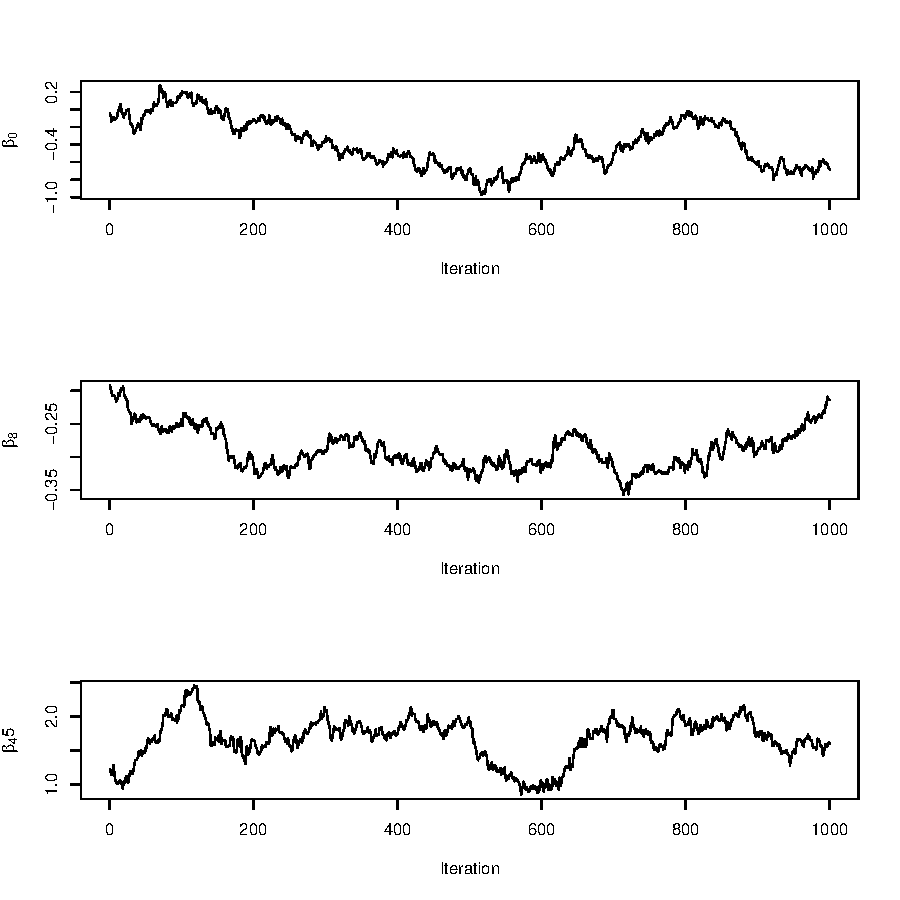
\includegraphics[width=1\textwidth]{traceplot_poisson_zip_da.pdf}
 \caption{Trace plots of three parameters from DA ZIP model}
 \end{subfigure}
  \hfill 
 \begin{subfigure}[b]{0.45\textwidth}
 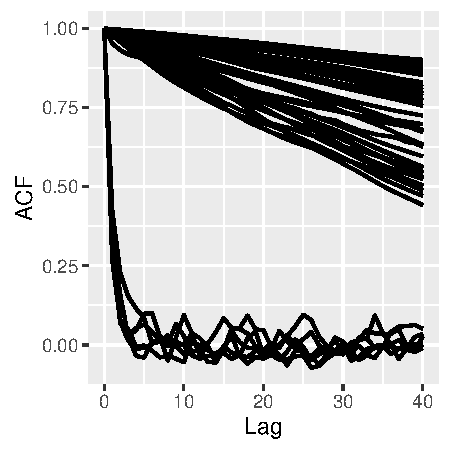
\includegraphics[width=1\textwidth]{poisson_zip_da_acf.pdf}
 \caption{Autocorrelation of all the 96 $\theta$'s from DA ZIP model.}
 \end{subfigure}  
 \caption{The hierarchy in the zero-inflated Poisson model does NOT help reduce the autocorrelation.}
 \end{figure}



\subsection{Goodness-of-Fit and Cross-Validation for Poisson Regression}


 \begin{figure}[H]
 % \centering
   \begin{subfigure}[b]{0.45\textwidth}
 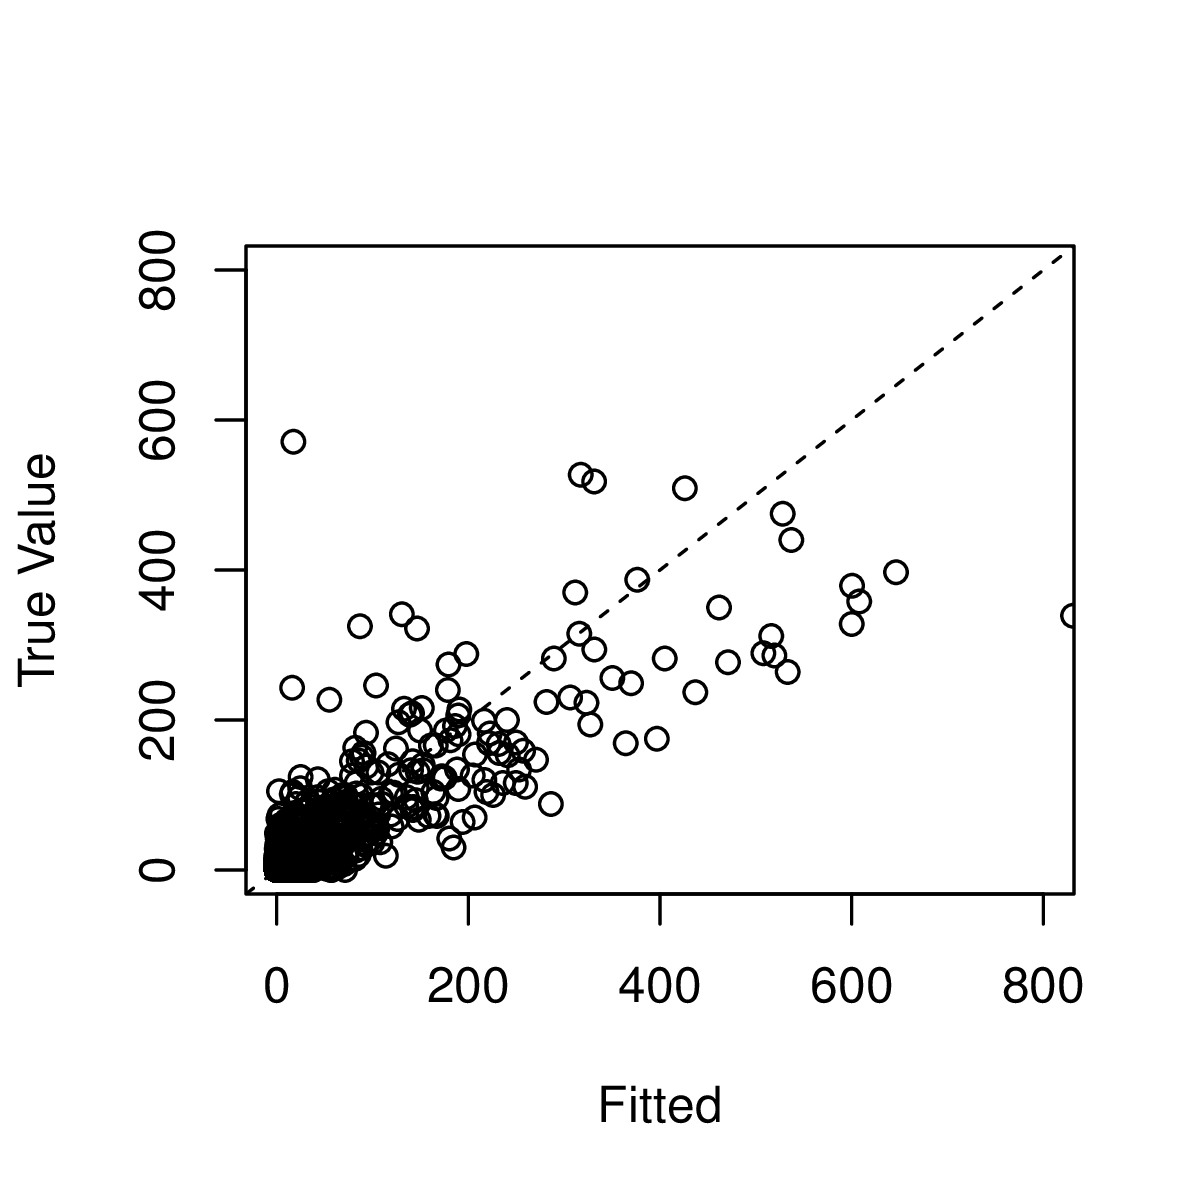
\includegraphics[width=1\textwidth]{poisson_fitting_da.png}
 \caption{Fitted vs true values using DA}
 \end{subfigure}
  \hfill 
 \begin{subfigure}[b]{0.45\textwidth}
 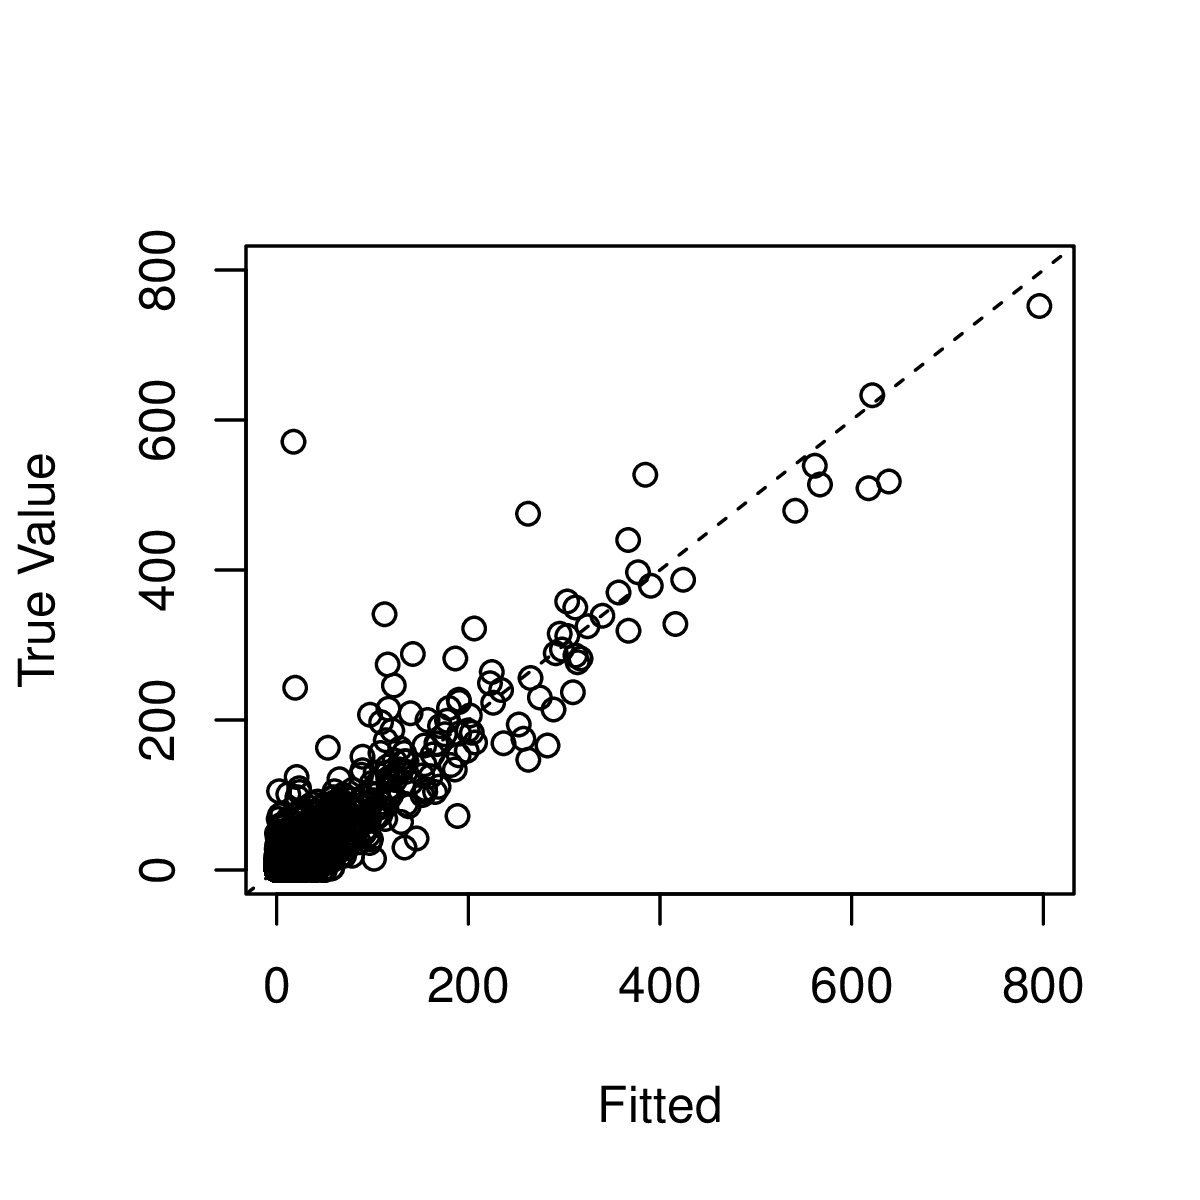
\includegraphics[width=1\textwidth]{poisson_fitting_ada.png}
 \caption{Fitted vs true values using CDA}
 \end{subfigure}  
   \begin{subfigure}[b]{0.45\textwidth}
 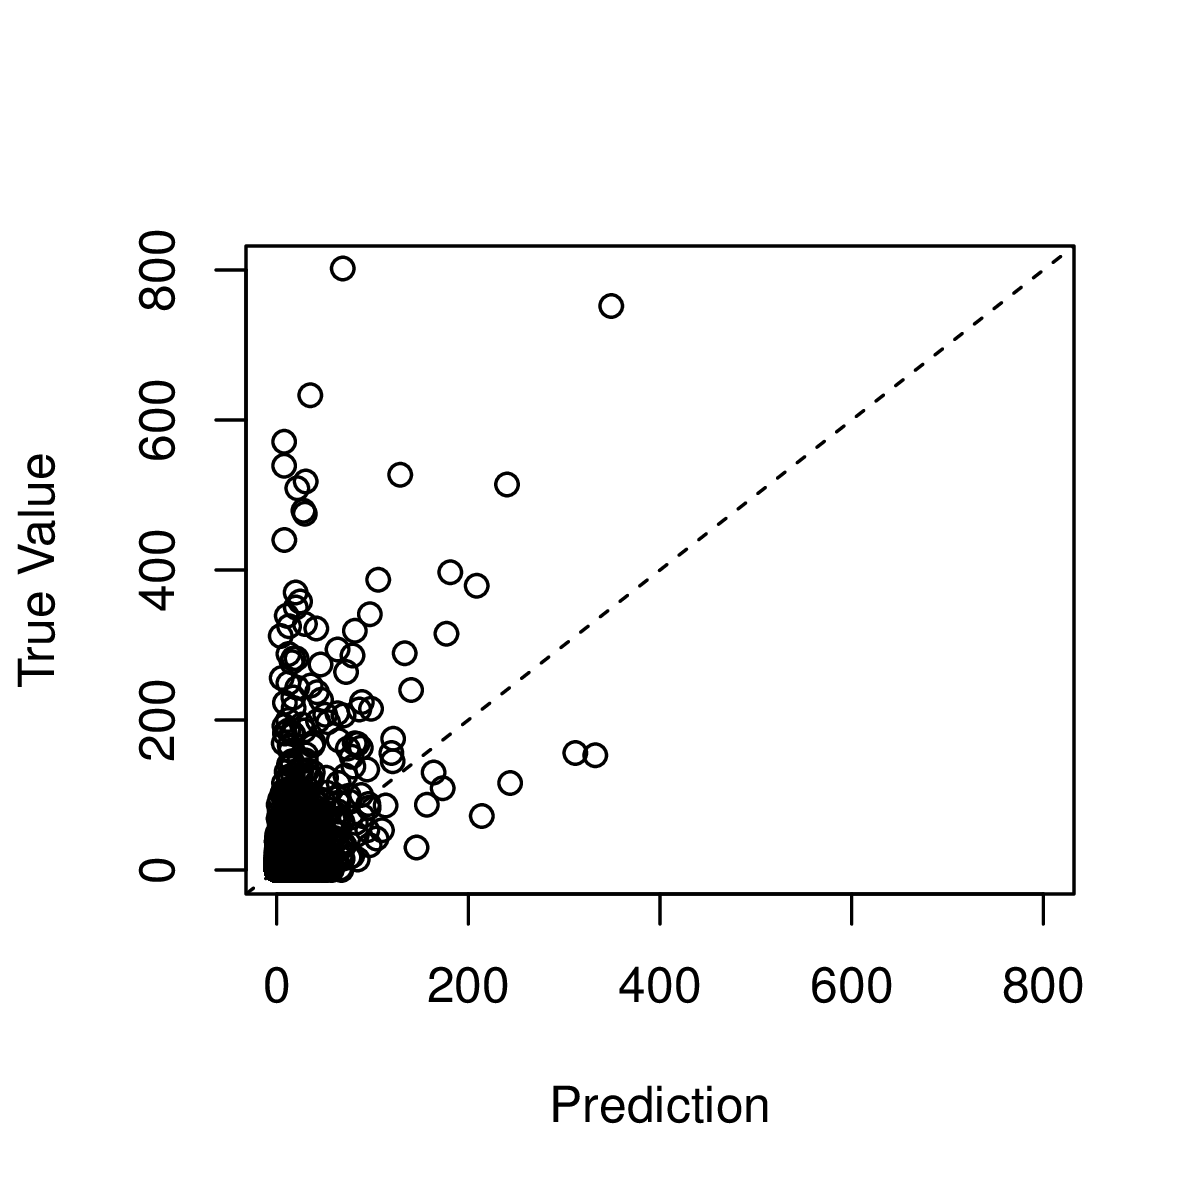
\includegraphics[width=1\textwidth]{poisson_cv_da.png}
 \caption{Prediction vs true values using DA}
 \end{subfigure}
  \hfill 
 \begin{subfigure}[b]{0.45\textwidth}
 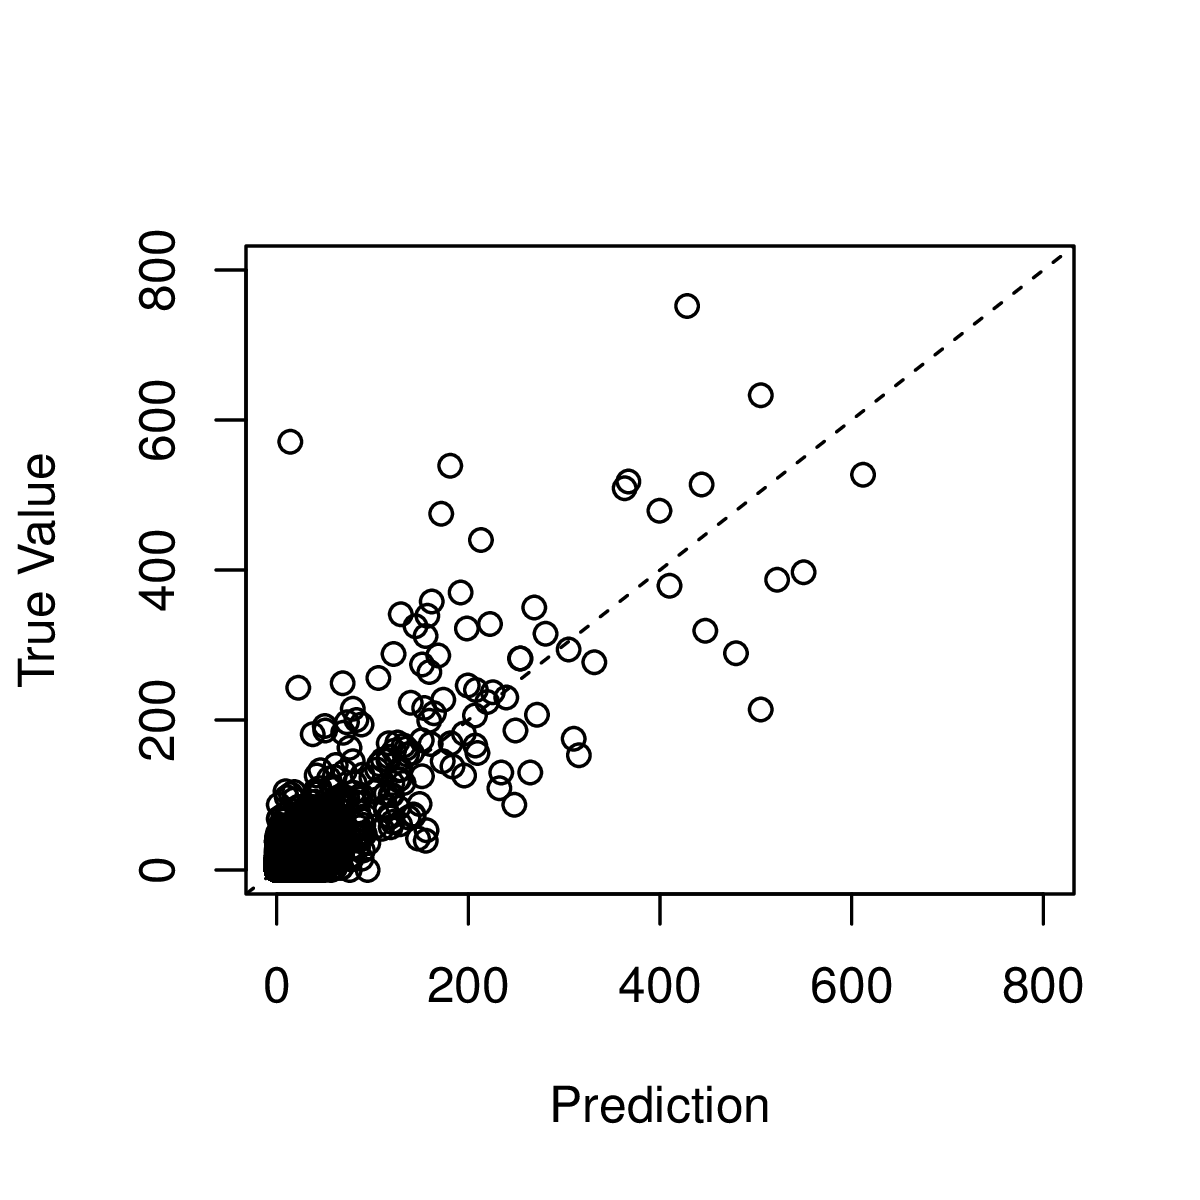
\includegraphics[width=1\textwidth]{poisson_cv_ada.png}
 \caption{Prediction vs true values using CDA}
 \end{subfigure} 
 \caption{The posterior estimates produced by CDA is better fitted to the data and have more accurate prediction than DA.}
 \end{figure}

 \subsection{Comparing posterior samples of CDA with HMC}


\begin{figure}[H]
 % \centering
   \begin{subfigure}[b]{0.45\textwidth}
 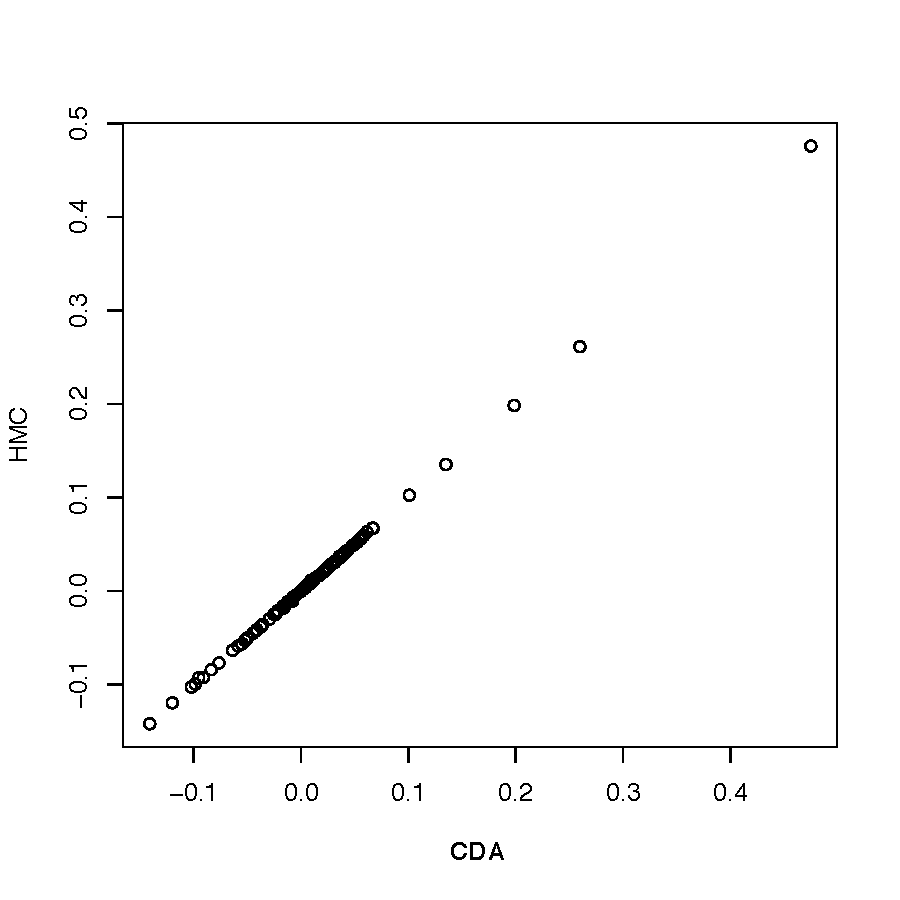
\includegraphics[width=1\textwidth]{CDAvsHMC_mean.pdf}
 \caption{Comparing posterior means for $\theta_1,\dots \theta_{95}$ from the HMC and CDA. The  RMSE between the two is $0.0007$.}
 \end{subfigure}
  \hfill 
 \begin{subfigure}[b]{0.45\textwidth}
 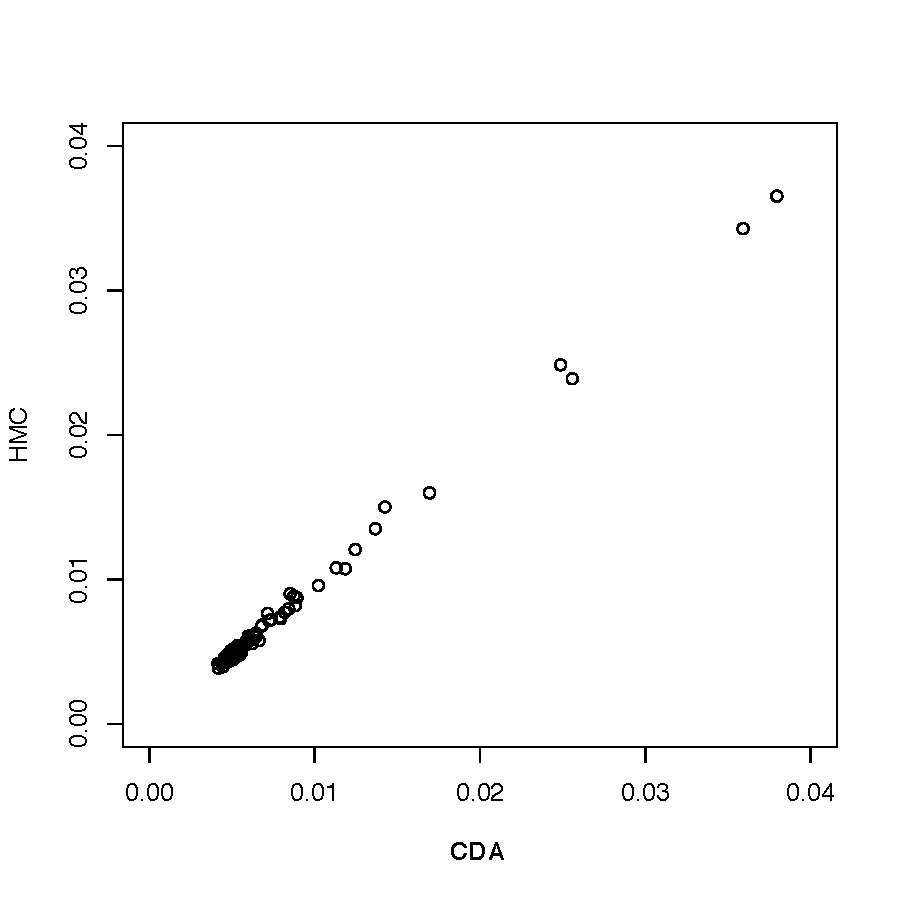
\includegraphics[width=1\textwidth]{CDAvsHMC_sd.pdf}
 \caption{Comparing posterior standard deviation for $\theta_1,\dots \theta_{95}$ from the HMC and CDA.  The  RMSE between the two is $0.0004$.}
 \end{subfigure}  
 \caption{The results from CDA and HMC agree very well.}
 \end{figure}

\subsection{Mixing of HMC}


 \begin{figure}[H]
 % \centering
   \begin{subfigure}[b]{0.45\textwidth}
 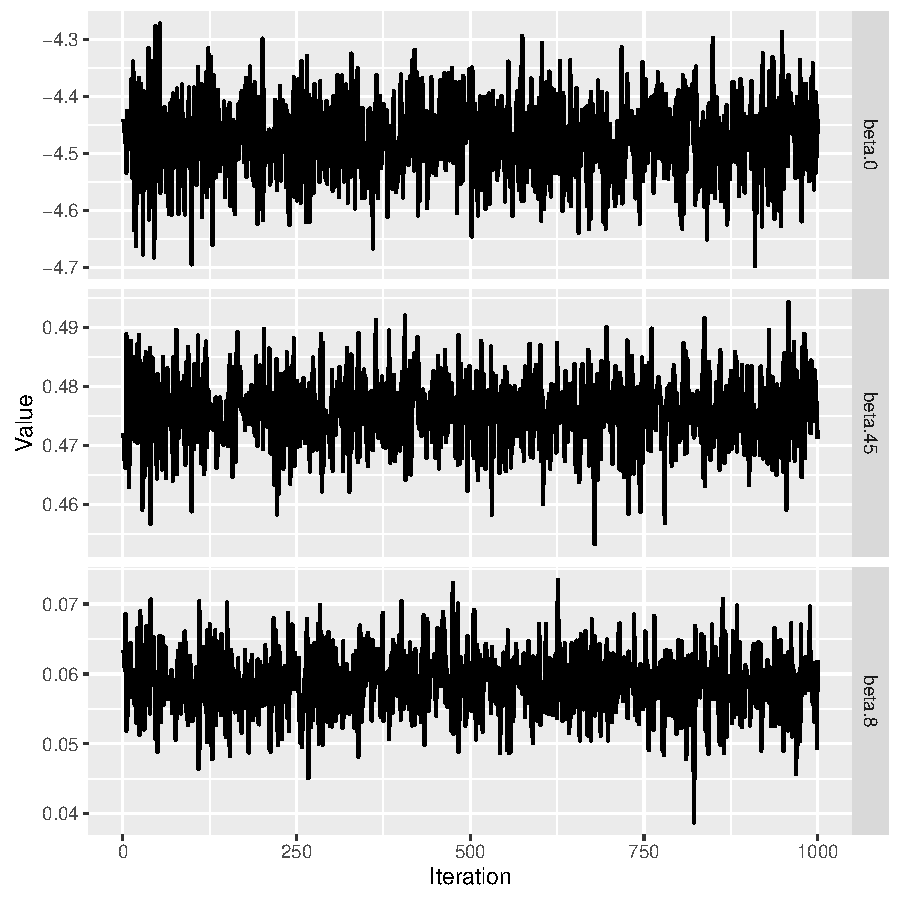
\includegraphics[width=1\textwidth]{traceplot_poisson_hmc.pdf}
 \caption{Traceplots}
 \end{subfigure}
  \hfill 
 \begin{subfigure}[b]{0.45\textwidth}
 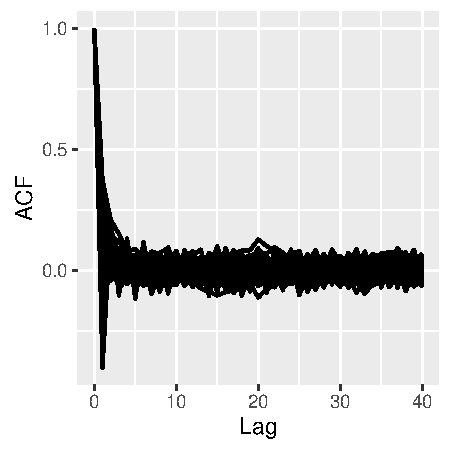
\includegraphics[width=1\textwidth]{poisson_hmc_acf.pdf}
 \caption{Autocorrelation}
 \end{subfigure}  
 \caption{The posterior estimates produced by HMC.}
 \end{figure}
 


 
\end{document}




